% This is samplepaper.tex, a sample chapter demonstrating the
% LLNCS macro package for Springer Computer Science proceedings;
% Version 2.21 of 2022/01/12
%
\documentclass[runningheads]{llncs}
%
\usepackage[T1]{fontenc}
% T1 fonts will be used to generate the final print and online PDFs,
% so please use T1 fonts in your manuscript whenever possible.
% Other font encondings may result in incorrect characters.
%

% Graphics and Figures
\usepackage{graphicx} % For images
\usepackage{float} % Helps with precise figure placement
\usepackage{subfig}  % For subfloats
\usepackage{cite}


\usepackage{comment}
\usepackage{amsmath}

\newtheorem{observation}{Observation}


% Math Symbols and Formatting
\usepackage{amssymb} % Additional math symbols


% Algorithms (LNCS does not include algorithm packages)
\usepackage{algorithm} % Algorithm floating environment
\usepackage{algorithmic} % Algorithm pseudocode formatting
\usepackage{subfloat}
% Bold Math
\usepackage{bm} % For bold math symbols

% TikZ for Diagrams (Not included in LNCS)
\usepackage{tikz}
\usetikzlibrary{shapes.geometric, positioning, calc, arrows, automata, shapes.misc} 

% Multiple Columns (if needed)
\usepackage{multicol} 

% Custom Macros for Problem Statements
\newcommand{\probleminput}[1]{\textit{Input:} #1}
\newcommand{\problemquestion}[1]{\textit{Question:} #1}

% Bibliography Format (LNCS does not use natbib)
\bibliographystyle{splncs04} 


\begin{document}
%
\title{Minimal non-comparability graphs and semi-transitivity}
%
%\titlerunning{Abbreviated paper title}
% If the paper title is too long for the running head, you can set
% an abbreviated paper title here




%
\author{Benny George Kenkireth \and
Gopalan Sajith \and
Sreyas Sasidharan}
%
\authorrunning{Kenkireth et al.}
% First names are abbreviated in the running head.
% If there are more than two authors, 'et al.' is used.
%
\institute{Department of Computer Science and Engineering, IIT Guwahati, India \\
\email{ben@iitg.ac.in, sajith@iitg.ac.in, sreyas.s@iitg.ac.in}}

%
\maketitle              % typeset the header of the contribution
%
\begin{abstract}

The concept of word-representable graphs has been widely explored in the literature. The class of word-representable graphs is characterized by the existence of a semi-transitive orientation. Specifically, a graph is word-representable if and only if it admits such an orientation. Comparability graphs form a subclass of word-representable graphs. Both word-representable and comparability graphs belong to hereditary graph classes. Every hereditary class can be characterized in terms of their forbidden induced subgraphs. The minimal forbidden induced subgraphs of comparability graphs and word-representable graphs are referred to as minimal non-comparability graphs and minimal non-word-representable graphs, respectively. 
    \paragraph{}
While the complete set of minimal non-comparability graphs is known, identifying the set of all minimal non-word-representable graphs remains an open problem. In this paper, we precisely determine the set of all minimal non-comparability graphs that are minimal non-word-representable graphs as well. To achieve this, we categorize all minimal non-comparability graphs into those that are semi-transitive and those that are not. 
 \paragraph{}
Furthermore, as a byproduct of our classification, we establish a characterization and a complete list of minimal non-word-representable graphs that contain an all-adjacent vertex. This is accomplished by introducing an all-adjacent vertex to each minimal non-comparability graph that is semi-transitive. As a result of our study, we identify several infinite families of minimal non-word-representable graphs, expanding the understanding of their structural properties.


%The abstract should briefly summarize the contents of the paper in
%150--250 words.

\keywords{comparability graph \and minimal non-comparability graph \and word-representable graph \and minimal non-word-representable graph \and semi-transitivity.}
\end{abstract}





\section{Introduction}

\paragraph{Comparability Graphs}  
Comparability graphs form an important class of graphs characterized by the existence of a transitive orientation. These are graphs whose edges can be oriented such that for any three vertices \(x\), \(y\), and \(z\), if there is a directed edge from \(x\) to \(y\) and from \(y\) to \(z\), then a directed edge from \(x\) to \(z\) exists. Comparability graphs belong to hereditary graph classes. A graph class \(X\) is said to be hereditary if, for any graph in \(X\), all of its induced subgraphs also belong to \(X\). Every hereditary graph class can be characterized in terms of forbidden induced subgraphs \cite{book}. The list of minimal forbidden induced subgraphs for comparability graphs was identified by Gallai in \cite{Gallai1967TransitivOG}. These graphs, known as minimal non-comparability graphs, do not admit a transitive orientation, but every proper induced subgraph of them does.


\paragraph{Word-representable graphs and semi-transitivity}
A graph is said to be \textit{word-representable} if there exists a word over its vertex set such that two vertices are adjacent if and only if their occurrences alternate within the word. The notion of word-representable graphs was introduced by Sergey Kitaev in \cite{perkins}. Since its inception, this concept has garnered significant attention (\cite{newres}, \cite{kitaev2017comprehensive}, \cite{onrepgraphs}). Word-representable graphs hold significance within graph theory, as they encompass various graph classes such as $3$-colorable graphs, sub-cubic graphs, and comparability graphs \cite{book}. Word-representable graphs also belong to hereditary graph classes.  However, the identification of the complete set of minimal forbidden induced subgraphs (also called minimal non-word-representable graphs) for word-representable graphs remains an open problem. Word-representable graphs are characterized by the existence of a semi-transitive orientation. Specifically, a graph is word-representable if and only if it admits such an orientation \cite{Halldorsson2011}. The notion of semi-transitivity extends the concept of transitive orientations. A graph is said to be semi-transitive if it admits an acyclic orientation satisfying a specific ordering condition on directed paths.
 \paragraph{}
We address the following question in this paper.
\begin{problem}
Are there minimal non-comparability graphs that also qualify as minimal non-word-representable graphs? If so, which graphs belong to this intersection?
\end{problem}

\paragraph{Contributions} In this paper, we determine which minimal non-comparability graphs are also minimal non-word-representable graphs. We establish that this intersection consists of two infinite families of graphs and a graph on $7$ vertices. To identify this intersection, we classify all minimal non-comparability graphs into those that are semi-transitive and those that are not. Building on this classification, we identify and characterize minimal non-word-representable graphs containing an all-adjacent vertex.  As a result, we identify several infinite families of minimal non-word-representable graphs.


\paragraph{Organization}

The paper is organized as follows. In Section \ref{section-prelims}, we provide the basic definitions and results that we follow in this paper. In Section \ref{section-min-semi-trans}, we identify the minimal non-comparability graphs, which are semi-transitive. In Section \ref{section-minimal-non-semi-trans}, we identify the minimal non-comparability graphs, which are not semi-transitive. Section \ref{section-conclusion} provides the concluding remarks.



\section{Preliminaries}
\label{section-prelims}
The graphs that we consider in this paper are all simple graphs. For a graph $G$, $V(G)$ denotes the vertex set of $G$, and $E(G)$ denotes the edge set of $G$. 

\begin{definition}
Consider a word $w$ on the alphabet $\Sigma$. For any $i,j \in \Sigma$, the word $w_{ij}$ is the word $w$ restricted to the copies of $i$ and $j$ in the order of their appearance in $w$. The letters $i$ and $j$ are said to alternate in $w$ if there is no substring of the form $ii$ or $jj$ in the word $w_{ij}$.
\end{definition}

\begin{example}
    Let $w=3123143$. The letters $1$ and $2$ alternate in $w$, as the substrings $11$ and $22$ are absent in $w_{12}=121$. The letters $1$ and $3$ are alternating in $w$, as $w_{13}=31313$. Letters $2$ and $4$ alternate in $w$, as $w_{24}=24$. Letters $2$ and $3$ does not alternate in $w$, as $w_{23}=3233$, and it has a substring $33$ in it. Letters $1$ and $4$ are not alternating in $w$, as $w_{14}=114$ contains the substring $11$ in it. Letters $3$ and $4$ are not alternating in $w$, as $w_{34}=3343$ contains the substring $33$ in it.
\end{example}


\begin{definition}
    A graph $G$ is said to be word-representable if there exists a word $w$ over $V(G)$ such that for any distinct pair of vertices $i,j \in V(G)$, $\{i,j\} \in E(G)$ if and only if the letters $i$ and $j$ alternate in $w$. The word $w$ is said to represent $G$.
\end{definition}

\begin{figure}[htbp]
    \centering
    \subfloat[$G_{1}$]{
        \centering
        % First figure
        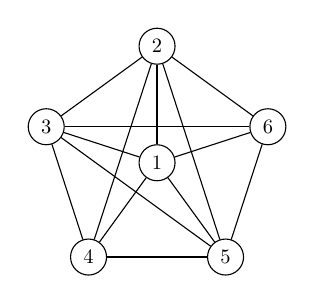
\begin{tikzpicture}[scale=0.74, transform shape]
            % TikZ code for the first figure


                 \centering
      \tikzset{vertex/.style = {shape=circle,draw=black,minimum size=1.5em}}
        \tikzset{edge/.style = {draw=black, - = latex'}}
    % vertices
    
        \node[vertex, text=black] (1) at  (0, 0) {$1$};
        \node[vertex, text=black] (2) at  (90:2cm) {$2$};
        \node[vertex, text=black] (3) at  (162:2cm) {$3$};
        \node[vertex, text=black] (4) at  (234:2cm) {$4$};
        \node[vertex, text=black] (5) at  (306:2cm) {$5$};
        \node[vertex, text=black] (6) at  (378:2cm) {$6$};
    
       \draw[edge] (1) to node[label= above:] {} (2); 
        \draw[edge] (1) to node[label= above:] {} (3); 
		 \draw[edge] (1) to node[label= right:] {}(4);        
          \draw[edge] (6) to node[label= right:] {}(1);
        \draw[edge] (5) to node[label= right:] {}(1);
        \draw[edge] (2) to node[label= left: ] {}(3);
        \draw[edge] (2) to node[label= right:] {}(6);
        \draw[edge] (6) to node[label= right:] {}(5);
       
        \draw[edge] (5) to node[label= right:] {}(4);
         \draw[edge] (4) to node[label= right:] {}(3);
        \draw[edge] (5) to node[label= right:] {}(3);
         \draw[edge] (5) to node[label= right:] {}(2);
        \draw[edge] (2) to node[label= right:] {}(4);
         \draw[edge] (3) to node[label= right:] {}(6);
        
            
        \end{tikzpicture}
    %    \caption{C}
        \label{fig:g(w)}
  }
  \hfill
    \subfloat[$G_{2}$]{
        \centering
        % Second figure
        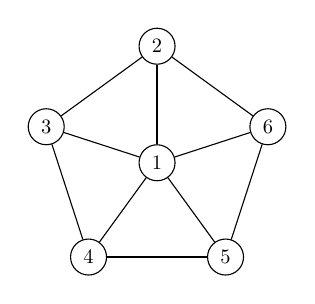
\begin{tikzpicture}[scale=0.74, transform shape]
            % TikZ code for the second figure
                     \centering
      \tikzset{vertex/.style = {shape=circle,draw=black,minimum size=1.5em}}
        \tikzset{edge/.style = {draw=black, - = latex'}}
    % vertices
    
        \node[vertex, text=black] (1) at  (0, 0) {$1$};
        \node[vertex, text=black] (2) at  (90:2cm) {$2$};
        \node[vertex, text=black] (3) at  (162:2cm) {$3$};
        \node[vertex, text=black] (4) at  (234:2cm) {$4$};
        \node[vertex, text=black] (5) at  (306:2cm) {$5$};
        \node[vertex, text=black] (6) at  (378:2cm) {$6$};
        
       \draw[edge] (1) to node[label= above:] {} (2); 
        \draw[edge] (1) to node[label= above:] {} (3); 
		 \draw[edge] (1) to node[label= right:] {}(4);        
          \draw[edge] (6) to node[label= right:] {}(1);
        \draw[edge] (5) to node[label= right:] {}(1);
        \color{red}
        \draw[edge] (2) to node[label= left: ] {}(3);
        \draw[edge] (2) to node[label= right:] {}(6);
        \draw[edge] (6) to node[label= right:] {}(5);
       
        \draw[edge] (5) to node[label= right:] {}(4);
         \draw[edge] (4) to node[label= right:] {}(3);
        \end{tikzpicture}
       % \caption{$G_{2}$}
        \label{fig:examplenon-wr}
    }
    \caption{$G_{1}$ is a word-representable graph and $G_{2}$ is a non-word-representable graph. }
    \label{fig:combined_word_rep_non_word_rep}
\end{figure}

\begin{example}
   The graph $G_{1}$ in Figure \ref{fig:g(w)} is an example of a word-representable graph. The word $w=6123564$ represents $G_{1}$. The graph $G_{2}$ in Figure \ref{fig:examplenon-wr} is the Wheel graph $W_{5}$ on six vertices. 
\end{example}

\begin{definition}
    A class of graphs $X$ is said to be hereditary if, for any graph $G \in X$, all induced subgraphs of $G$ belong to the class $X$.
\end{definition}

\begin{example}
    Planar graphs, comparability graphs, and word-representable graphs are all examples of hereditary graph classes.
\end{example}

The class of word-representable graphs is hereditary\cite{book}, which implies that any induced subgraph of a word-representable graph is word-representable. One of the important properties of hereditary graph classes is that they admit forbidden induced subgraph characterization.

\begin{definition}
    A graph \( G \) is a forbidden induced subgraph for a hereditary class \( X \) if \( G \) is not an induced subgraph of any graph \( H \in X \). This means that no graph in \( X \) can have \( G \) as an induced subgraph.
\end{definition}

\begin{example}
    Wheel graph $W_{5}$ shown in Figure \ref{fig:minimal} is a forbidden induced subgraph for word-representable graphs. $W_{5}$ is also a minimal forbidden induced subgraph for the class of word-representable graphs.
\end{example}

\begin{definition}
    A graph $G$ is a minimal forbidden induced subgraph for a hereditary class $X$ if $G$ is a forbidden induced subgraph for $X$ and if any proper induced subgraph of $G$ belongs to $X$.
\end{definition}

There exists a unique set of minimal forbidden induced subgraphs for every hereditary class $X$ \cite{book}. The minimal forbidden induced subgraphs for word-representable graphs are the minimal non-word-representable graphs, and hence, it is of interest to study about them. 
\begin{definition}
\label{minimalandnonminimal}

Let $G$ be a non-word-representable graph. $G$ is a minimal non-word-representable graph if every proper induced subgraph of $G$ is word-representable. 

   % A minimal non-word-representable graph $G$ is a non-word-representable graph having all of its induced subgraphs as word-representable. A non-minimal non-word-representable graph has at least one non-word-representable induced subgraph present in it.
\end{definition}


\begin{figure}[h]
    \centering
    \subfloat[$G_{1}$]{
        \centering
        % First figure
        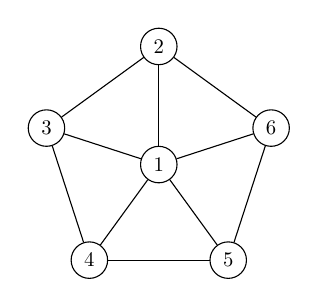
\begin{tikzpicture}[scale=0.75, transform shape]
            % TikZ code for the first figure


                 \centering
      \tikzset{vertex/.style = {shape=circle,draw=black,minimum size=1.5em}}
        \tikzset{edge/.style = {draw=black, - = latex'}}
    % vertices
    
        \node[vertex, text=black] (1) at  (0, 0) {$1$};
        \node[vertex, text=black] (2) at  (90:2cm) {$2$};
        \node[vertex, text=black] (3) at  (162:2cm) {$3$};
        \node[vertex, text=black] (4) at  (234:2cm) {$4$};
        \node[vertex, text=black] (5) at  (306:2cm) {$5$};
        \node[vertex, text=black] (6) at  (378:2cm) {$6$};
    
       \draw[edge] (1) to node[label= above:] {} (2); 
        \draw[edge] (1) to node[label= above:] {} (3); 
		 \draw[edge] (1) to node[label= right:] {}(4);        
          \draw[edge] (6) to node[label= right:] {}(1);
        \draw[edge] (5) to node[label= right:] {}(1);
        \draw[edge] (2) to node[label= left: ] {}(3);
        \draw[edge] (2) to node[label= right:] {}(6);
        \draw[edge] (6) to node[label= right:] {}(5);
       
        \draw[edge] (5) to node[label= right:] {}(4);
         \draw[edge] (4) to node[label= right:] {}(3);
       
        
            
        \end{tikzpicture}
     %   \caption{$G_{1}$}
        \label{fig:minimal}
 }
 \hfill
    \subfloat[$G_{2}$]{
        \centering
        % Second figure
        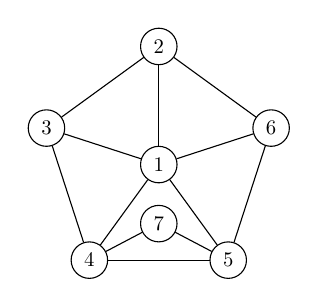
\begin{tikzpicture}[scale=0.75, transform shape]
            % TikZ code for the second figure
                     \centering
      \tikzset{vertex/.style = {shape=circle,draw=black,minimum size=1.5em}}
        \tikzset{edge/.style = {draw=black, - = latex'}}
    % vertices
    
        \node[vertex, text=black] (1) at  (0, 0) {$1$};
        \node[vertex, text=black] (2) at  (90:2cm) {$2$};
        \node[vertex, text=black] (3) at  (162:2cm) {$3$};
        \node[vertex, text=black] (4) at  (234:2cm) {$4$};
        \node[vertex, text=black] (5) at  (306:2cm) {$5$};
        \node[vertex, text=black] (6) at  (378:2cm) {$6$};
         \node[vertex, text=black] (7) at  (0,-1) {$7$};
        
       \draw[edge] (1) to node[label= above:] {} (2); 
        \draw[edge] (1) to node[label= above:] {} (3); 
		 \draw[edge] (1) to node[label= right:] {}(4);        
          \draw[edge] (6) to node[label= right:] {}(1);
        \draw[edge] (5) to node[label= right:] {}(1);
    
        \draw[edge] (2) to node[label= left: ] {}(3);
        \draw[edge] (2) to node[label= right:] {}(6);
        \draw[edge] (6) to node[label= right:] {}(5);
       \draw[edge] (4) to node[label= left: ] {}(7);
       %\draw[edge] (1) to node[label= left: ] {}(7);
       \draw[edge] (5) to node[label= left: ] {}(7);
       
        \draw[edge] (5) to node[label= right:] {}(4);
         \draw[edge] (4) to node[label= right:] {}(3);
         
        \end{tikzpicture}
        %\caption{$G_{2}$}
        \label{fig:non-minimal}
    }
    \caption{$G_{1}$ is minimal non-word-representable graph, where as $G_{2}$ is non-minimal non-word-representable graph.}
    \label{fig:combined_minimal_non_minimal}
\end{figure}


\begin{example}
     The graph $G_{1}$ in Figure \ref{fig:minimal} is an example of a minimal non-word-representable graph. $G_{1}$ is the Wheel graph $W_{5}$ on six vertices. The graph $G_{2}$ in Figure \ref{fig:non-minimal} contains Wheel graph $W_{5}$ as an induced subgraph, and hence $G_{2}$ is a non-minimal non-word-representable graph.
\end{example}



The notion of semi-transitivity is very important in the study of word-representable graphs.  

\begin{definition}
\label{semi-trans-defn}
A graph $G$ is semi-transitive if it admits an acyclic orientation such that for any directed path $v_{1} \rightarrow v_{2} \rightarrow \cdots \rightarrow v_{k}$, with $v_{i} \in V(G)$, either 
\begin{itemize}
    \item there is no edge $v_{1} \rightarrow v_{k}$, or
    \item the edge $v_{1} \rightarrow v_{k}$ is present and there are edges $v_{i} \rightarrow v_{j}$, for all $1 \leq i<j \leq k$.
\end{itemize}
    Such an orientation is called semi-transitive orientation. The property of having a semi-transitive orientation is referred to as the semi-transitivity property.
\end{definition}

\begin{note}
    A directed path $P = v_{1} \rightarrow v_{2} \rightarrow \cdots \rightarrow v_{k}$ is said to violate semi-transitivity if the edge $v_{1} \rightarrow v_{k}$ exists, but there is at least one missing edge $v_{i} \rightarrow v_{j}$ for some $1 \leq i < j \leq k$. A directed graph $G$ is semi-transitive if it is acyclic, and no path in $G$ violates semi-transitivity.
\end{note}


\begin{example}
    An example of a semi-transitive orientation is shown in Figure \ref{fig:semi-trans}. Observe that the longest path of the graph in Figure \ref{fig:semi-trans} is of length $3$, which is the path $3 \rightarrow 2 \rightarrow 6 \rightarrow 1$. Since $6 \rightarrow 1$ is not an edge, it does not violate the semi-transitivity. One thing to note is that any directed path of length $2$ will not be a violation of semi-transitivity. It does not matter if there exists an edge between the first vertex and the third vertex in the path.

\begin{figure}[h]
\begin{center}
        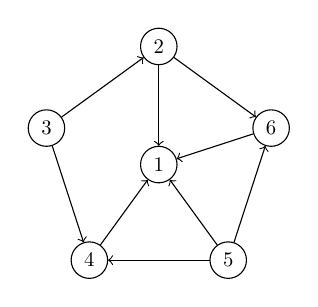
\begin{tikzpicture}[scale=0.75, transform shape]
            % TikZ code for the first figure


                 \centering
      \tikzset{vertex/.style = {shape=circle,draw=black,minimum size=1.5em}}
        \tikzset{edge/.style = {draw=black, -> = latex'}}
    % vertices
    
        \node[vertex, text=black] (1) at  (0, 0) {$1$};
        \node[vertex, text=black] (2) at  (90:2cm) {$2$};
        \node[vertex, text=black] (3) at  (162:2cm) {$3$};
        \node[vertex, text=black] (4) at  (234:2cm) {$4$};
        \node[vertex, text=black] (5) at  (306:2cm) {$5$};
        \node[vertex, text=black] (6) at  (378:2cm) {$6$};
    
       \draw[edge ] (2) to node[label= above:] {} (1); 
        
		 \draw[edge] (4) to node[label= right:] {}(1);        
          \draw[edge] (6) to node[label= right:] {}(1);
        \draw[edge] (5) to node[label= right:] {}(1);
        \draw[edge] (3) to node[label= left: ] {}(2);
        \draw[edge] (2) to node[label= right:] {}(6);
        \draw[edge] (5) to node[label= right:] {}(6);
       
        \draw[edge] (5) to node[label= right:] {}(4);
         \draw[edge] (3) to node[label= right:] {}(4);
       
        
            
        \end{tikzpicture}
        \end{center}
        \caption{A semi-transitive orientation.}
        \label{fig:semi-trans}
        \end{figure}

\end{example}

Theorem \ref{wrg=semi} is significant as it establishes that a graph is word-representable if and only if it is semi-transitive. This result suggests that to prove a graph $G$ is word-representable, it is sufficient to demonstrate that $G$ is semi-transitive.
\begin{theorem}
\cite{book}
\label{wrg=semi}
    A graph $G$ is word-representable if and only if it admits a semi-transitive orientation.
\end{theorem}


\begin{definition}
    Let \( G \) be a directed graph and \( v \in V(G) \). The vertex \( v \) is called a \emph{source vertex} if all edges incident to \( v \) are directed away from it. Similarly, \( v \) is called a \emph{sink vertex} if all edges incident to \( v \) are directed towards it.
\end{definition}


\begin{example}
    Consider the Figure \ref{fig:semi-trans}. $1$ is a sink vertex, and $3$ is a source vertex.
\end{example}



Theorem \ref{source_vertex} is an interesting result about the existence of semi-transitive orientations with any vertex as the source.

\begin{theorem}
\label{source_vertex}
\cite{kitaev2023humanverifiable}
    If a graph $G$ is word-representable, then there is a semi-transitive orientation of $G$ with any vertex $v \in V(G)$ as a source vertex.
\end{theorem}

Theorem \ref{3-col_is_semi} states that any $3$-colorable graph is word-representable.
\begin{theorem}
\label{3-col_is_semi}
\cite{Halldorsson2011}
    Any $3$-colorable graph $G$ is semi-transitive.
\end{theorem}


\begin{definition}
    A graph $G$ is a comparability graph if and only if the edges of $G$ admit a transitive orientation. That is, if there is an edge directed from $a$ to $b$ and an edge directed from $b$ to $c$, then there is an edge directed from $a$ to $c$. A graph $G$, which is not a comparability graph, is called a non-comparability graph.
\end{definition}


\begin{example}
    \begin{figure}[h]
        \centering
        \subfloat[$G_{1}$]{
            \centering
           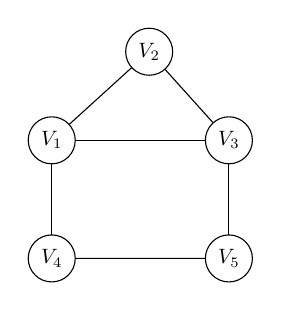
\begin{tikzpicture}[scale=0.75, transform shape]
                \tikzset{edge/.style = {->,> = latex'}}
                \tikzset{vertex/.style = {shape=circle,draw,minimum size=1.5em}}
                \tikzset{edge/.style = {-,> = latex'}}
                % vertices
                \node[vertex] (1) at  (-1.5, -1.5) {$V_{1}$};
                \node[vertex] (2) at  (0.15, 0) {$V_{2}$};
                \node[vertex] (3) at  (1.5,-1.5) {$V_{3}$};
                \node[vertex] (4) at  (-1.5, -3.5) {$V_{4}$};
                \node[vertex] (5) at  (1.5, -3.5) {$V_{5}$};
                \draw[edge] (1) to (2); 
                \draw[edge] (2) to (3);
                \draw[edge] (3) to (5);
                \draw [edge] (1) to (4);      
                \draw [edge] (5) to (4);    
                \draw [edge] (1) to (3);  
            \end{tikzpicture}
           % \caption{$G_{1}$}
            \label{fig:comp-graph}
        }
        \hfill
         \subfloat[A transitive orientation of $G_{1}$]{
            \centering
            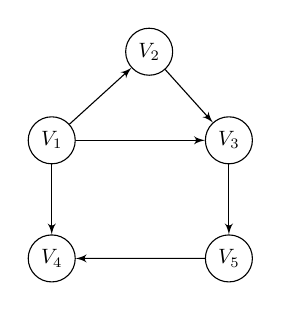
\begin{tikzpicture}[scale=0.75, transform shape]
                \tikzset{edge/.style = {->,> = latex'}}
                \tikzset{vertex/.style = {shape=circle,draw,minimum size=1.5em}}
                \tikzset{edge/.style = {->,> = latex'}}
                % vertices
                \node[vertex] (1) at  (-1.5, -1.5) {$V_{1}$};
                \node[vertex] (2) at  (0.15, 0) {$V_{2}$};
                \node[vertex] (3) at  (1.5,-1.5) {$V_{3}$};
                \node[vertex] (4) at  (-1.5, -3.5) {$V_{4}$};
                \node[vertex] (5) at  (1.5, -3.5) {$V_{5}$};
                \draw[edge] (1) to (2); 
                \draw[edge] (2) to (3);
                \draw[edge] (3) to (5);
                \draw [edge] (1) to (4);      
                \draw [edge] (5) to (4);    
                    \draw [edge] (1) to (3); 
            \end{tikzpicture}
            %\caption{A transitive orientation of $G_{1}$}
            \label{fig:trans-orient-comp-graph}
        }
        \hfill
        \subfloat[$G_{2}$]{
            \centering
            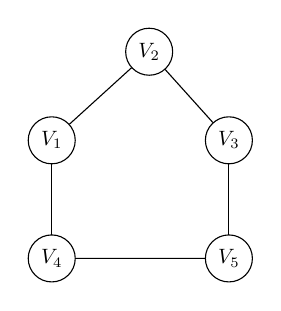
\begin{tikzpicture}[scale=0.75, transform shape]
                \tikzset{edge/.style = {->,> = latex'}}
                \tikzset{vertex/.style = {shape=circle,draw,minimum size=1.5em}}
                \tikzset{edge/.style = {-,> = latex'}}
                % vertices
                 \node[vertex] (1) at  (-1.5, -1.5) {$V_{1}$};
                \node[vertex] (2) at  (0.15, 0) {$V_{2}$};
                \node[vertex] (3) at  (1.5,-1.5) {$V_{3}$};
                \node[vertex] (4) at  (-1.5, -3.5) {$V_{4}$};
                \node[vertex] (5) at  (1.5, -3.5) {$V_{5}$};
                \draw[edge] (1) to (2); 
                \draw[edge] (2) to (3);
                \draw[edge] (3) to (5);
                \draw [edge] (1) to (4);      
                \draw [edge] (5) to (4);    
            \end{tikzpicture}
         %   \caption{$G_{2}$}
            \label{fig:non-comp-graph}
        }
        \caption{$G_{1}$ is a comparability graph and $G_{2}$ is a non-comparability graph.}
    \end{figure}
    Figure \ref{fig:comp-graph} shows an example of a comparability graph, and Figure \ref{fig:trans-orient-comp-graph} provides one of its transitive orientations. $G_{2}$ in Figure \ref{fig:non-comp-graph} is $C_{5}$, which is known to be a non-comparability graph \cite{Gallai1967TransitivOG}.
\end{example}

Comparability graphs form a subclass of word-representable graphs \cite{book}. The class of comparability graphs is hereditary, and hence, a forbidden induced subgraph characterization exists. In the case of comparability graphs, the set of all minimal forbidden induced subgraphs $($minimal non-comparability graphs$)$ is known and was discovered by Gallai in \cite{Gallai1967TransitivOG}. 

\begin{definition}
    Let $G$ be a non-comparability graph. $G$ is said to be a minimal non-comparability graph if every proper induced subgraph of $G$ is a comparability graph. If $G$ is not a minimal non-comparability graph, then $G$ is a non-minimal non-comparability graph.
\end{definition}

 \begin{example}
    \begin{figure}[h]
        \centering
        \subfloat[$G_{1}$]{
            \centering
            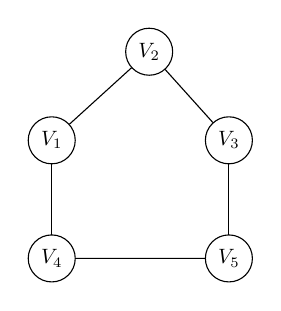
\begin{tikzpicture}[scale=0.75, transform shape]
                \tikzset{edge/.style = {->,> = latex'}}
                \tikzset{vertex/.style = {shape=circle,draw,minimum size=1.5em}}
                \tikzset{edge/.style = {-,> = latex'}}
                % vertices
                \node[vertex] (1) at  (-1.5, -1.5) {$V_{1}$};
                \node[vertex] (2) at  (0.15, 0) {$V_{2}$};
                \node[vertex] (3) at  (1.5,-1.5) {$V_{3}$};
                \node[vertex] (4) at  (-1.5, -3.5) {$V_{4}$};
                \node[vertex] (5) at  (1.5, -3.5) {$V_{5}$};
                \draw[edge] (1) to (2); 
                \draw[edge] (2) to (3);
                \draw[edge] (3) to (5);
                \draw [edge] (1) to (4);      
                \draw [edge] (5) to (4);    
            \end{tikzpicture}
           % \caption{$G_{1}$}
            \label{fig:minimal-comp-graph}
        }
        \hfill
        \subfloat[$G_{2}$]{
            \centering
            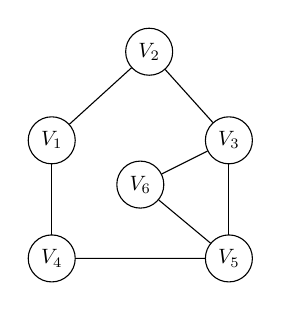
\begin{tikzpicture}[scale=0.75, transform shape]
                \tikzset{edge/.style = {->,> = latex'}}
                \tikzset{vertex/.style = {shape=circle,draw,minimum size=1.5em}}
                \tikzset{edge/.style = {-,> = latex'}}
                % vertices
               \node[vertex] (1) at  (-1.5, -1.5) {$V_{1}$};
                \node[vertex] (2) at  (0.15, 0) {$V_{2}$};
                \node[vertex] (3) at  (1.5,-1.5) {$V_{3}$};
                \node[vertex] (4) at  (-1.5, -3.5) {$V_{4}$};
                \node[vertex] (5) at  (1.5, -3.5) {$V_{5}$};
                \node[vertex] (6) at  (0, -2.25) {$V_{6}$};  % Corrected duplicate label
                \draw[edge] (1) to (2); 
                \draw[edge] (2) to (3);
                \draw[edge] (3) to (5);
                \draw [edge] (1) to (4);      
                \draw [edge] (5) to (4);    
                \draw[edge] (3) to (6);
                \draw[edge] (6) to (5);
            \end{tikzpicture}
          %  \caption{$G_{2}$}
            \label{fig:non-minimal-non-comp-graph}
        }
        \caption{$G_{1}$ is a minimal non-comparability graph and $G_{2}$ is non-minimal non-comparability graph.}
    \end{figure}

    Figure \ref{fig:minimal-comp-graph} shows $C_{5}$, which is known to be a minimal non-comparability graph \cite{Gallai1967TransitivOG}, and since $G_{2}$ in Figure \ref{fig:non-minimal-non-comp-graph} contains $G_{1}$ as a proper induced subgraph, $G_{2}$ is a non-minimal non-comparability graph. 
\end{example}

Gallai provided the forbidden induced subgraph characterization for comparability graphs in \cite{Gallai1967TransitivOG}. Gallai identified the complete list of minimal forbidden induced subgraphs for comparability graphs, which are precisely what we call minimal non-comparability graphs. The list of all minimal non-comparability graphs is given in Figure \ref{fig:min-non-comp-part1},  \ref{fig:min-non-comp-part2}, \ref{fig:min-non-comp-part3}, and \ref{fig:min-non-comp-part4}. 
\paragraph{}
Several infinite classes of graphs are illustrated in Figures \ref{fig:min-non-comp-part1}, \ref{fig:min-non-comp-part2}, and \ref{fig:min-non-comp-part3}. The individual graphs that are minimal non-comparability graphs are shown in Figure \ref{fig:min-non-comp-part4}. In particular, Figure \ref{fig:min-non-comp-part2} presents two distinct classes of graphs, where only the missing edges are highlighted. Dashed edges represent absent connections, while all other edges are present.  Additionally, Figure \ref{fig:min-non-comp-part3} depicts three graph classes, each structured into three levels. Given the complexity of these graphs, dashed edges are used in certain levels to indicate the only missing edges within that level. All other edges in the induced subgraph of vertices at that level remain present.

\begin{figure}[htbp]
    \centering
    \subfloat[$G_{n}^{1}=\{C_{2n+1}~; ~n \geq 2\}$]{
%for cycle 2n+1.
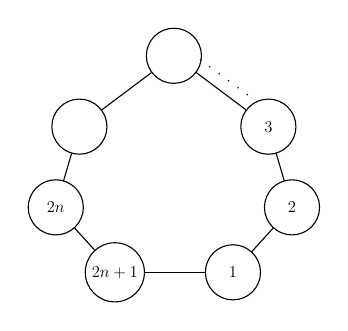
\begin{tikzpicture}[scale=0.5, transform shape, every node/.style={font=\large}]

\node[draw, circle, minimum size=1.4cm] (1) at (2, 0) {$1$};
\node[draw, circle, minimum size=1.4cm] (2) at (3.5, 1.65) {$2$};
\node[draw, circle, minimum size=1.4cm] (3) at (2.9, 3.7) {$3$};
\node[draw, circle, minimum size=1.4cm] (r) at (0.5, 5.5) {};
\node[draw, circle, minimum size=1.4cm] (r1) at (-1.9, 3.7) {};
\node[draw, circle, minimum size=1.4cm] (2n) at (-2.5, 1.65) {$2n$};
\node[draw, circle, minimum size=1.4cm] (2n+1) at (-1, 0) {$2n+1$};

\draw[-] (1) -- (2);
\draw[-] (2) -- (3);
\draw[-] (3) -- (r) node[midway, sloped, above, yshift=5pt] {. . . . . . .}; % Label shifted a bit upward
\draw[-] (r) -- (r1);
\draw[-] (r1) -- (2n);
\draw[-] (2n) -- (2n+1);
\draw[-] (2n+1) -- (1);

\end{tikzpicture}
 %\subcaption{$G_{n}^{1}=\{C_{2n+1}~; ~n \geq 2\}$}
 \label{g1n}
}
\hfill
\subfloat[$G_{n}^{2}$ $;$ $n \geq 2$]{
        % Second TikZ picture
 
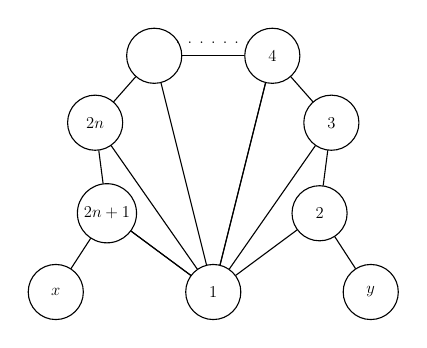
\begin{tikzpicture}[scale=0.5, transform shape, every node/.style={font=\large}]

\node[draw, circle, minimum size=1.4cm] (1) at (0, -2) {$1$};
\node[draw, circle, minimum size=1.4cm] (2) at (2.7, 0) {$2$};
\node[draw, circle, minimum size=1.4cm] (2n+1) at (-2.7, 0) {$2n+1$};
\node[draw, circle, minimum size=1.4cm] (3) at (3, 2.3) {$3$};
\node[draw, circle, minimum size=1.4cm] (4) at (1.5, 4) {$4$};
\node[draw, circle, minimum size=1.4cm] (r) at (-1.5, 4) {};
\node[draw, circle, minimum size=1.4cm] (2n) at (-3, 2.3) {$2n$};
\node[draw, circle, minimum size=1.4cm] (x) at (-4, -2) {$x$};
\node[draw, circle, minimum size=1.4cm] (y) at (4, -2) {$y$};

\draw[-] (1) -- (2);
\draw[-] (2) -- (3);
\draw[-] (3) -- (4);
\draw[-] (4) -- (r) node[midway, above, yshift=5pt] {. . . . . . .};
\draw[-] (r) -- (2n);
\draw[-] (2n) -- (2n+1);
\draw[-] (2n+1) -- (1);
\draw[-] (1) -- (3);
\draw[-] (1) -- (4);
\draw[-] (1) -- (4);
\draw[-] (1) -- (r);
\draw[-] (1) -- (2n);
\draw[-] (1) -- (2n+1);
\draw[-] (2n+1) -- (x);
\draw[-] (2) -- (y);

\end{tikzpicture}
 %   \subcaption{$G_{n}^{2}$ $;$ $n \geq 2$}
    \label{g2n}
}
    
    \vspace{0.6cm} % Space between the two rows

\subfloat[$G_{n}^{3}$ $;$ $n \geq 3$]{
        % Third TikZ picture
     
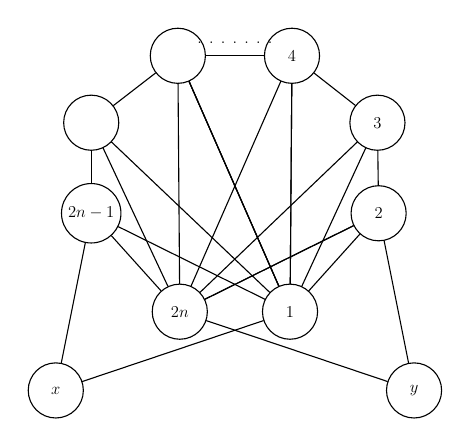
\begin{tikzpicture}[scale=0.5, transform shape, every node/.style={font=\large}]

\node[draw, circle, minimum size=1.4cm] (1) at (1.15, -2.5) {$1$};
\node[draw, circle, minimum size=1.4cm] (2) at (3.4, 0) {$2$};
\node[draw, circle, minimum size=1.4cm] (2n-1) at (-3.9, 0) {$2n-1$};
\node[draw, circle, minimum size=1.4cm] (3) at (3.37, 2.3) {$3$};
\node[draw, circle, minimum size=1.4cm] (r1) at (-3.9, 2.3) {};
\node[draw, circle, minimum size=1.4cm] (4) at (1.2, 4) {$4$};
\node[draw, circle, minimum size=1.4cm] (r) at (-1.7, 4) {};
\node[draw, circle, minimum size=1.4cm] (2n) at (-1.65, -2.5) {$2n$};
\node[draw, circle, minimum size=1.4cm] (x) at (-4.8, -4.5) {$x$};
\node[draw, circle, minimum size=1.4cm] (y) at (4.3, -4.5) {$y$};

\draw[-] (1) -- (2);
\draw[-] (2) -- (3);
\draw[-] (3) -- (4);
\draw[-] (4) -- (r) node[midway, above, yshift=5pt] {. . . . . . .};
\draw[-] (1) -- (3);
\draw[-] (1) -- (4);
\draw[-] (1) -- (4);
\draw[-] (1) -- (r);
\draw[-] (1) -- (r);
\draw[-] (1) -- (r1);
\draw[-] (1) -- (2n-1);
\draw[-] (1) -- (r);
\draw[-] (2n) -- (2);
\draw[-] (2n) -- (3);
\draw[-] (2n) -- (4);
\draw[-] (2n) -- (r);
\draw[-] (2n) -- (r1);
\draw[-] (2n) -- (2n-1);
\draw[-] (2n) -- (2);
\draw[-] (r) -- (r1);
\draw[-] (2n-1) -- (r1);
\draw[-] (2n-1) -- (x);
\draw[-] (2) -- (y);
\draw[-] (2n) -- (y);
\draw[-] (1) -- (x);

\end{tikzpicture}

 %\subcaption{$G_{n}^{3}$ $;$ $n \geq 3$}
 \label{g3n}
}
 \hfill
\subfloat[$G_{n}^{4}$ $;$ $n \geq 3$]{
        % Fourth TikZ picture
  
            % Your fourth TikZ code here
  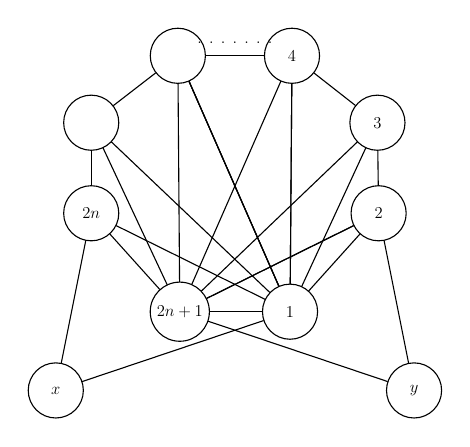
\begin{tikzpicture}[scale=0.5, transform shape, every node/.style={font=\large}]

\node[draw, circle, minimum size=1.4cm] (1) at (1.15, -2.5) {$1$};
\node[draw, circle, minimum size=1.4cm] (2) at (3.4, 0) {$2$};
\node[draw, circle, minimum size=1.4cm] (2n) at (-3.9, 0) {$2n$};
\node[draw, circle, minimum size=1.4cm] (3) at (3.37, 2.3) {$3$};
\node[draw, circle, minimum size=1.4cm] (r1) at (-3.9, 2.3) {};
\node[draw, circle, minimum size=1.4cm] (4) at (1.2, 4) {$4$};
\node[draw, circle, minimum size=1.4cm] (r) at (-1.7, 4) {};
\node[draw, circle, minimum size=1.4cm] (2n+1) at (-1.65, -2.5) {$2n+1$};
\node[draw, circle, minimum size=1.4cm] (x) at (-4.8, -4.5) {$x$};
\node[draw, circle, minimum size=1.4cm] (y) at (4.3, -4.5) {$y$};

\draw[-] (1) -- (2);
\draw[-] (2) -- (3);
\draw[-] (3) -- (4);
\draw[-] (4) -- (r) node[midway, above, yshift=5pt] {. . . . . . .};
\draw[-] (1) -- (3);
\draw[-] (1) -- (4);
\draw[-] (1) -- (4);
\draw[-] (1) -- (r);
\draw[-] (1) -- (r);
\draw[-] (1) -- (r1);
\draw[-] (1) -- (2n);
\draw[-] (1) -- (r);
\draw[-] (1) -- (2n+1);
\draw[-] (2n+1) -- (2);
\draw[-] (2n+1) -- (3);
\draw[-] (2n+1) -- (4);
\draw[-] (2n+1) -- (r);
\draw[-] (2n+1) -- (r1);
\draw[-] (2n+1) -- (2n);
\draw[-] (2n+1) -- (2);
\draw[-] (r) -- (r1);
\draw[-] (2n) -- (r1);
\draw[-] (2n) -- (x);
\draw[-] (2) -- (y);
\draw[-] (2n+1) -- (y);
\draw[-] (1) -- (x);

\end{tikzpicture}
 %\subcaption{$G_{n}^{4}$ $;$ $n \geq 3$}
 \label{g4n}
}
    
  \caption{Minimal non-comparability graphs - $1$ $($Four infinite classes of graphs.$)$}
  \label{fig:min-non-comp-part1}
\end{figure}
\begin{figure}[htbp]
    \centering
    \subfloat[$G_{n}^{5}$ $;$ $n \geq 3$]{
        \centering
        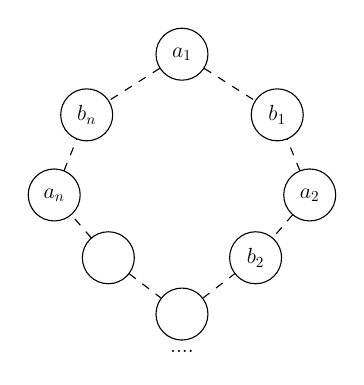
\begin{tikzpicture}[scale=0.55, transform shape, every node/.style={font=\Large}]
            % First Graph
            \node[draw, circle, minimum size=1.2cm] (a1) at (0, 4) {$a_{1}$};
            \node[draw, circle, minimum size=1.2cm] (b1) at (2.2, 2.6) {$b_{1}$};
            \node[draw, circle, minimum size=1.2cm] (a2) at (2.95, 0.75) {$a_{2}$};
            \node[draw, circle, minimum size=1.2cm] (b2) at (1.7, -0.7) {$b_{2}$};
            \node[draw, circle, minimum size=1.2cm] (r) at (0, -2) {};
            \node[below= 0.1cm of r] {....};
            \node[draw, circle, minimum size=1.2cm] (r1) at (-1.7, -0.7) {};
            \node[draw, circle, minimum size=1.2cm] (an) at (-2.95, 0.75) {$a_{n}$};
            \node[draw, circle, minimum size=1.2cm] (bn) at (-2.2, 2.6) {$b_{n}$};
            
            \draw[-, dashed] (a1) -- (b1);
            \draw[-, dashed] (a2) -- (b1);
            \draw[-, dashed] (a2) -- (b2);
            \draw[-, dashed] (r) -- (b2);
            \draw[-, dashed] (r1) -- (r);
            \draw[-, dashed] (r1) -- (an);
            \draw[-, dashed] (an) -- (bn);
            \draw[-, dashed] (a1) -- (bn);
        \end{tikzpicture}
        \label{g5n}
    }
    \hfill
    \subfloat[$G_{n}^{6}$ $;$ $n \geq 3$]{
        \centering
        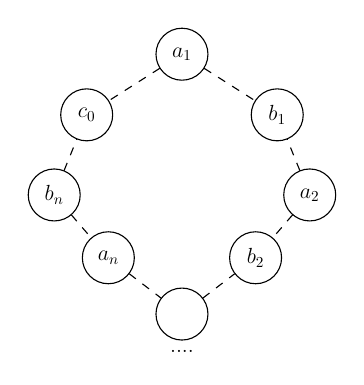
\begin{tikzpicture}[scale=0.55, transform shape, every node/.style={font=\Large}]
            % Second Graph
            \node[draw, circle, minimum size=1.2cm] (a1) at (0, 4) {$a_{1}$};
            \node[draw, circle, minimum size=1.2cm] (b1) at (2.2, 2.6) {$b_{1}$};
            \node[draw, circle, minimum size=1.2cm] (a2) at (2.95, 0.75) {$a_{2}$};
            \node[draw, circle, minimum size=1.2cm] (b2) at (1.7, -0.7) {$b_{2}$};
            \node[draw, circle, minimum size=1.2cm] (r) at (0, -2) {};
            \node[below= 0.1cm of r] {....};
            \node[draw, circle, minimum size=1.2cm] (an) at (-1.7, -0.7) {$a_{n}$};
            \node[draw, circle, minimum size=1.2cm] (bn) at (-2.95, 0.75) {$b_{n}$};
            \node[draw, circle, minimum size=1.2cm] (c0) at (-2.2, 2.6) {$c_{0}$};
            
            \draw[-, dashed] (a1) -- (c0);
            \draw[-, dashed] (bn) -- (c0);
            \draw[-, dashed] (a2) -- (b1);
            \draw[-, dashed] (a2) -- (b2);
            \draw[-, dashed] (r) -- (b2);
            \draw[-, dashed] (an) -- (r);
            \draw[-, dashed] (bn) -- (an);
            \draw[-, dashed] (a1) -- (b1);
        \end{tikzpicture}
        \label{g6n}
    }
    \caption{Minimal non-comparability graphs - $2$ $($Two infinite classes of graphs, where only the missing edges are highlighted. Dashed edges represent absent connections, while all other edges are present.$)$}
    \label{fig:min-non-comp-part2}
\end{figure}

\begin{figure}[htbp]
    \centering
    % First subfigure in the first row
    \subfloat[$G_{n}^{7}$ $;$ $n \geq 1$]{
        \centering
        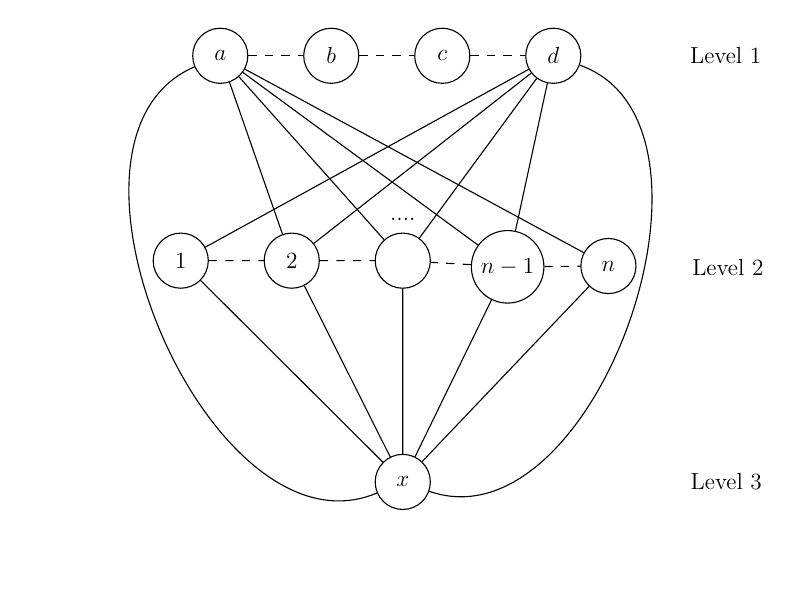
\begin{tikzpicture}[scale=0.7, transform shape, every node/.style={font=\large}]
            % Graph 1
            % Nodes with the same radius
            \node[draw, circle,  minimum size=1cm] (a) {$a$};
            \node[draw, circle,  right=of a, minimum size=1cm] (b) {$b$};
            \node[draw, circle,  right=of b, minimum size=1cm] (c) {$c$};
            \node[draw, circle,  right=of c, minimum size=1cm] (d) {$d$};

            % Increased vertical distance for the second row
            \node[draw, circle,  below left=of a, minimum size=1cm, xshift= 1cm, yshift=-2cm] (1) {$1$};
            \node[draw, circle,  below left=of b, minimum size=1cm, xshift= 1cm,  yshift=-2cm] (2) {$2$};

            \node[draw, circle, below left=of c, minimum size=1cm, xshift= 1cm, yshift=-2cm] (r) {}; 

            \node[above= 0.1cm of r] {....}; % Label 

            \node[draw, circle, below left=of d, minimum size=1cm, xshift= 1cm, yshift=-2cm] (n-1) {$n-1$}; 

            \node[draw, circle, below=of d, minimum size=1cm, xshift= 1cm, yshift=-1.8cm] (n) {$n$}; 

            % Increased vertical distance for the third row
            \node[draw, circle,  below=of r, minimum size=1cm, yshift=-2cm] (x) {$x$};

            % Edges with various styles
            \draw[-, dashed] (1) -- (2);
            \draw[-, dashed] (n-1) -- (r);
            \draw[-, dashed] (2) -- (r);
            \draw[-, dashed] (n-1) -- (n);
            \draw[-, dashed] (a) -- (b);
            \draw[-, dashed] (b) -- (c);
            \draw[-, dashed] (c) -- (d);

            \draw[-] (x) -- (1);
            \draw[-] (x) -- (2);
            \draw[-] (x) -- (n-1);
            \draw[-] (x) -- (n);
            \draw[-] (x) -- (r);

            \draw[-] (a) -- (n);
            \draw[-] (a) -- (2);
            \draw[-] (a) -- (n-1);
            \draw[-] (a) -- (r);

            \draw[-] (d) -- (1);
            \draw[-] (d) -- (2);
            \draw[-] (d) -- (n-1);
            \draw[-] (d) -- (r);

            \draw[-, bend left=90] (x) to (a);  % Sharper bend to the left
            \draw[-, bend right=90] (x) to (d); % Sharper bend to the right

            % Labels for the levels
            \node at ($(a)!1.39!(d)$) [right] {Level 1}; % Label for Level 1
            \node at ($(1)!1.18!(n)$) [right] {Level 2}; % Label for Level 2
            \node at ($(x)!2.5!(x)+(5.1,0)$) [right] {Level 3}; % Label for Level 3
        \end{tikzpicture}
        \label{g7n}
    }
    \hfill
    % Second subfigure in the first row
     \subfloat[$G_{n}^{8}$ $;$ $n \geq 1$]{
        \centering
        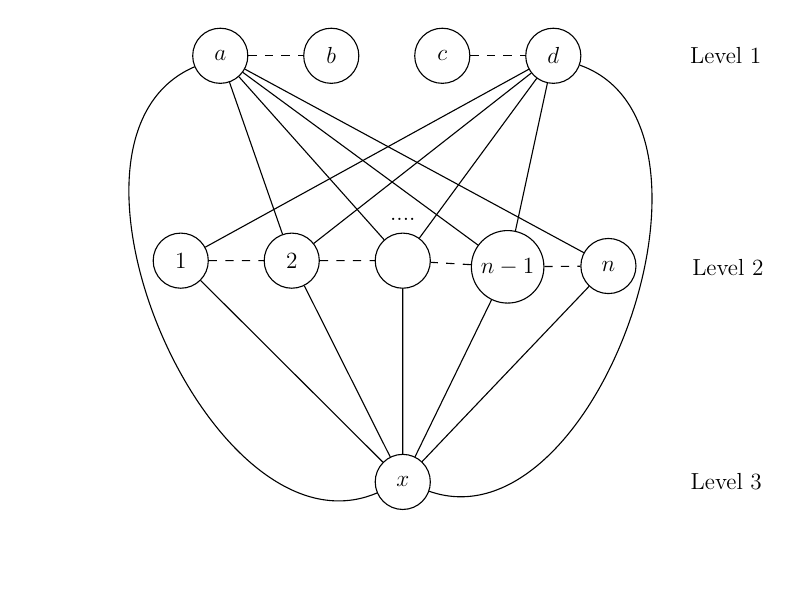
\begin{tikzpicture}[scale=0.7, transform shape, every node/.style={font=\large}]
            % Graph 1
            % Nodes with the same radius
            \node[draw, circle,  minimum size=1cm] (a) {$a$};
            \node[draw, circle,  right=of a, minimum size=1cm] (b) {$b$};
            \node[draw, circle,  right=of b, minimum size=1cm] (c) {$c$};
            \node[draw, circle,  right=of c, minimum size=1cm] (d) {$d$};

            % Increased vertical distance for the second row
            \node[draw, circle,  below left=of a, minimum size=1cm, xshift= 1cm, yshift=-2cm] (1) {$1$};
            \node[draw, circle,  below left=of b, minimum size=1cm, xshift= 1cm,  yshift=-2cm] (2) {$2$};

            \node[draw, circle, below left=of c, minimum size=1cm, xshift= 1cm, yshift=-2cm] (r) {}; 

            \node[above= 0.1cm of r] {....}; % Label 

            \node[draw, circle, below left=of d, minimum size=1cm, xshift= 1cm, yshift=-2cm] (n-1) {$n-1$}; 

            \node[draw, circle, below=of d, minimum size=1cm, xshift= 1cm, yshift=-1.8cm] (n) {$n$}; 

            % Increased vertical distance for the third row
            \node[draw, circle,  below=of r, minimum size=1cm, yshift=-2cm] (x) {$x$};

            % Edges with various styles
            \draw[-, dashed] (1) -- (2);
            \draw[-, dashed] (n-1) -- (r);
            \draw[-, dashed] (2) -- (r);
            \draw[-, dashed] (n-1) -- (n);
            \draw[-, dashed] (a) -- (b);
            
            \draw[-, dashed] (c) -- (d);

            \draw[-] (x) -- (1);
            \draw[-] (x) -- (2);
            \draw[-] (x) -- (n-1);
            \draw[-] (x) -- (n);
            \draw[-] (x) -- (r);

            \draw[-] (a) -- (n);
            \draw[-] (a) -- (2);
            \draw[-] (a) -- (n-1);
            \draw[-] (a) -- (r);

            \draw[-] (d) -- (1);
            \draw[-] (d) -- (2);
            \draw[-] (d) -- (n-1);
            \draw[-] (d) -- (r);

            \draw[-, bend left=90] (x) to (a);  % Sharper bend to the left
            \draw[-, bend right=90] (x) to (d); % Sharper bend to the right

            % Labels for the levels
            \node at ($(a)!1.39!(d)$) [right] {Level 1}; % Label for Level 1
            \node at ($(1)!1.18!(n)$) [right] {Level 2}; % Label for Level 2
            \node at ($(x)!2.5!(x)+(5.1,0)$) [right] {Level 3}; % Label for Level 3
        \end{tikzpicture}
        \label{g8n}
    }

    \vspace{0.5cm} % Space between rows

    % Third subfigure in the second row, centered
    \subfloat[$G_{n}^{9}$ $;$ $n \geq 2$]{
        \centering
        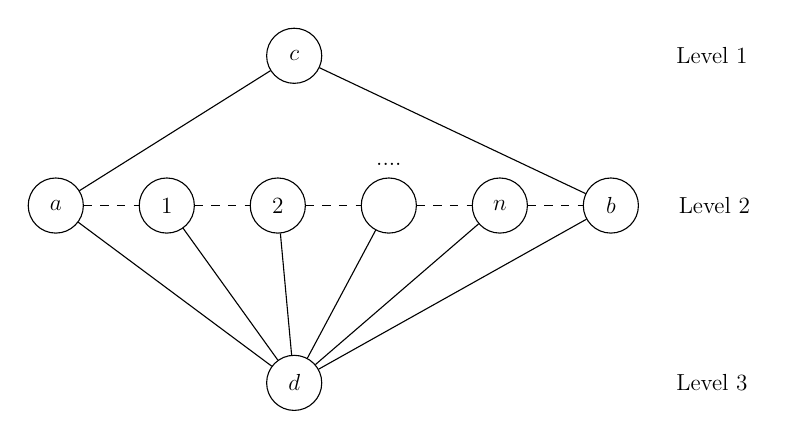
\begin{tikzpicture}[scale=0.7, transform shape, every node/.style={font=\large}]
            % Graph 3
            % Nodes with the same radius
            \node[draw, circle,  minimum size=1cm] (a) {$a$};
            \node[draw, circle,  right=of a, minimum size=1cm] (1) {$1$};
            \node[draw, circle,  right=of 1, minimum size=1cm] (2) {$2$};
            \node[draw, circle,  right=of 2, minimum size=1cm] (r) {};
            \node[above= 0.1cm of r] {....}; % Label 
            \node[draw, circle,  right=of r, minimum size=1cm] (n) {$n$};
            \node[draw, circle,  right=of n, minimum size=1cm] (b) {$b$};

            \node[draw, circle,  above left=of r, minimum size=1cm, yshift=1cm] (c) {$c$};

            % Increased vertical distance for the third row
            \node[draw, circle,  below left=of r, minimum size=1cm, yshift=-1.5cm] (d) {$d$};

            % Edges with various styles
            \draw[-, dashed] (a) -- (1);
            \draw[-, dashed] (1) -- (2);
            \draw[-, dashed] (2) -- (r);
            \draw[-, dashed] (r) -- (n);
            \draw[-, dashed] (n) -- (b);

            \draw[-] (d) -- (1);
            \draw[-] (d) -- (2);
            \draw[-] (d) -- (n);
            \draw[-] (d) -- (r);
            \draw[-] (d) -- (a);
            \draw[-] (d) -- (b);

            \draw[-] (a) -- (c);
            \draw[-] (c) -- (b);

            % Labels for the levels
            \node at ($(c)!1.39!(c)+(6.81,0)$) [right] {Level 1}; % Label for Level 1
            \node at ($(a)!1.11!(b)$) [right] {Level 2}; % Label for Level 2
            \node at ($(d)!2.5!(d)+(6.81,0)$) [right] {Level 3}; % Label for Level 3
        \end{tikzpicture}
        \label{g9n}
    }
    \caption{Minimal non-comparability graphs - $3$ (Three infinite graph classes, each structured into three levels. Due to the complexity of these graphs, dashed edges are used in certain levels to indicate the \textbf{only} missing edges within that level.)}
    \label{fig:min-non-comp-part3}
\end{figure}
\begin{figure}[htbp]
    \centering
    % First row
  \subfloat[$H_{1}$]{
        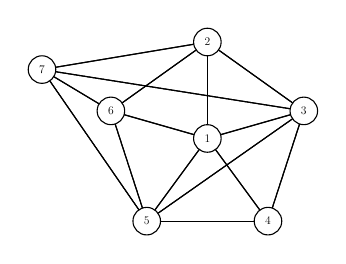
\begin{tikzpicture}[scale=0.35, transform shape, every node/.style={font=\large}]
        % Define nodes with coordinates
        \node[draw, circle, minimum size=1cm] (1) at (0, 0) {$1$};
        \node[draw, circle, minimum size=1cm] (2) at (-6, 2.5) {$7$};
        \node[draw, circle, minimum size=1cm] (3) at (2.2, -3) {$4$};
        \node[draw, circle, minimum size=1cm] (4) at (-3.5, 1) {$6$};
        \node[draw, circle, minimum size=1cm] (5) at (3.5, 1) {$3$};
        \node[draw, circle, minimum size=1cm] (6) at (0, 3.5) {$2$};
        \node[draw, circle, minimum size=1cm] (7) at (-2.2, -3) {$5$};

        % Draw edges based on the given connections
        \draw[-] (1) -- (3);
        \draw[-] (1) -- (4);
        \draw[-] (1) -- (5);
        \draw[-] (1) -- (6);
        \draw[-] (1) -- (7);
        \draw[-] (2) -- (4);
        \draw[-] (2) -- (5);
        \draw[-] (2) -- (6);
        \draw[-] (2) -- (7);
        \draw[-] (3) -- (1);
        \draw[-] (3) -- (5);
        \draw[-] (3) -- (7);
        \draw[-] (4) -- (1);
        \draw[-] (4) -- (2);
        \draw[-] (4) -- (6);
        \draw[-] (4) -- (7);
        \draw[-] (5) -- (1);
        \draw[-] (5) -- (2);
        \draw[-] (5) -- (3);
        \draw[-] (5) -- (6);
        \draw[-] (5) -- (7);
        \draw[-] (6) -- (1);
        \draw[-] (6) -- (2);
        \draw[-] (6) -- (4);
        \draw[-] (6) -- (5);
        \draw[-] (7) -- (1);
        \draw[-] (7) -- (2);
        \draw[-] (7) -- (3);
        \draw[-] (7) -- (4);
        \draw[-] (7) -- (5);
        \end{tikzpicture}
     %   \caption{$H_{1}$}
        \label{$H_{1}$}
   }
    \hfill
    \subfloat[$H_{2}$]{
        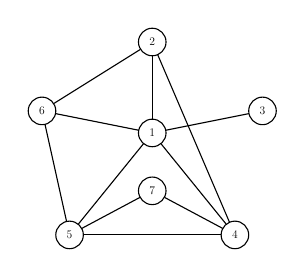
\begin{tikzpicture}[scale=0.35, transform shape, every node/.style={font=\large}]
        % Define nodes with coordinates
        \node[draw, circle, minimum size=1cm] (7) at (0, 0.2) {$1$};
        \node[draw, circle, minimum size=1cm] (4) at (0, -1.9) {$7$};
        \node[draw, circle, minimum size=1cm] (2) at (3, -3.5) {$4$};
        \node[draw, circle, minimum size=1cm] (3) at (-4, 1) {$6$};
        \node[draw, circle, minimum size=1cm] (1) at (4, 1) {$3$};
        \node[draw, circle, minimum size=1cm] (5) at (0, 3.5) {$2$};
        \node[draw, circle, minimum size=1cm] (6) at (-3, -3.5) {$5$};

        % Draw edges based on the given connections
        \draw[-] (7) -- (3);
        \draw[-] (7) -- (1);
        \draw[-] (7) -- (5);
        \draw[-] (7) -- (6);
        \draw[-] (7) -- (2);
        \draw[-] (2) -- (5);
        \draw[-] (2) -- (6);
        \draw[-] (3) -- (5);
        \draw[-] (3) -- (6);
        \draw[-] (4) -- (2);
        \draw[-] (4) -- (6);
        \end{tikzpicture}
      %  \caption{$H_{2}$}
        \label{$H_{2}$}
    }
    \hfill
    \subfloat[$H_{3}$]{
        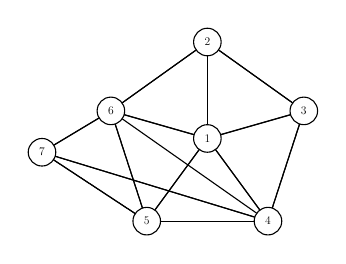
\begin{tikzpicture}[scale=0.35, transform shape, every node/.style={font=\large}]
        % Define nodes with coordinates
        \node[draw, circle, minimum size=1cm] (1) at (0, 0) {$1$};
        \node[draw, circle, minimum size=1cm] (2) at (-6, -0.5) {$7$};
        \node[draw, circle, minimum size=1cm] (6) at (2.2, -3) {$4$};
        \node[draw, circle, minimum size=1cm] (7) at (-3.5, 1) {$6$};
        \node[draw, circle, minimum size=1cm] (5) at (3.5, 1) {$3$};
        \node[draw, circle, minimum size=1cm] (3) at (0, 3.5) {$2$};
        \node[draw, circle, minimum size=1cm] (4) at (-2.2, -3) {$5$};

        % Draw edges based on the given connections
        \draw[-] (1) -- (3);
        \draw[-] (1) -- (4);
        \draw[-] (1) -- (5);
        \draw[-] (1) -- (6);
        \draw[-] (1) -- (7);
        \draw[-] (2) -- (4);
        \draw[-] (2) -- (6);
        \draw[-] (2) -- (7);
        \draw[-] (3) -- (1);
        \draw[-] (3) -- (5);
        \draw[-] (3) -- (7);
        \draw[-] (4) -- (1);
        \draw[-] (4) -- (2);
        \draw[-] (4) -- (6);
        \draw[-] (4) -- (7);
        \draw[-] (5) -- (1);
        \draw[-] (5) -- (3);
        \draw[-] (5) -- (6);
        \draw[-] (6) -- (1);
        \draw[-] (6) -- (2);
        \draw[-] (6) -- (4);
        \draw[-] (6) -- (5);
        \draw[-] (7) -- (1);
        \draw[-] (7) -- (2);
        \draw[-] (7) -- (3);
        \draw[-] (7) -- (4);
        \draw[-] (7) -- (6);
        \end{tikzpicture}
      %  \caption{$H_{3}$}
        \label{$H_{3}$}
    }
    
     \vspace{0.6cm} % space between rows
    \subfloat[$H_{4}$]{
        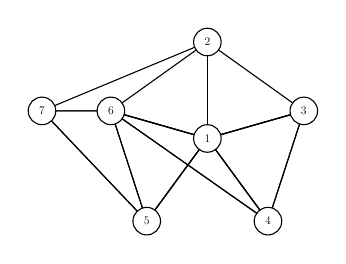
\begin{tikzpicture}[scale=0.35, transform shape, every node/.style={font=\large}]
       
        %add correct 4th here.
        
        % Define nodes with coordinates
\node[draw, circle, minimum size=1cm] (6) at (0, 0) {$1$};
\node[draw, circle, minimum size=1cm] (4) at (-6, 1) {$7$};
\node[draw, circle, minimum size=1cm] (2) at (2.2, -3) {$4$};
\node[draw, circle, minimum size=1cm] (7) at (-3.5, 1) {$6$};
\node[draw, circle, minimum size=1cm] (5) at (3.5, 1) {$3$};
\node[draw, circle, minimum size=1cm] (1) at (0, 3.5) {$2$};
\node[draw, circle, minimum size=1cm] (3) at (-2.2, -3) {$5$};

% Draw edges based on the given connections
\draw[-] (6) -- (1);
\draw[-] (6) -- (2);
\draw[-] (6) -- (3);
\draw[-] (6) -- (5);
\draw[-] (6) -- (7);

\draw[-] (2) -- (5);
\draw[-] (2) -- (6);
\draw[-] (2) -- (7);

\draw[-] (3) -- (4);
\draw[-] (3) -- (6);
\draw[-] (3) -- (7);

\draw[-] (4) -- (1);
\draw[-] (4) -- (3);
\draw[-] (4) -- (7);


\draw[-] (5) -- (1);
\draw[-] (5) -- (2);
\draw[-] (5) -- (6);


\draw[-] (6) -- (1);
\draw[-] (6) -- (2);
\draw[-] (6) -- (3);
\draw[-] (6) -- (5);
\draw[-] (6) -- (7);

\draw[-] (7) -- (1);
\draw[-] (7) -- (2);
\draw[-] (7) -- (3);
\draw[-] (7) -- (4);
\draw[-] (7) -- (6);

        \end{tikzpicture}
      %  \caption{$H_{4}$}
        \label{$H_{4}$}
    }
  \hfill
    \subfloat[$H_{5}$]{
        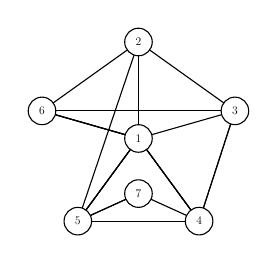
\begin{tikzpicture}[scale=0.35, transform shape, every node/.style={font=\large}]

        %add correct 5th here.
      % Define nodes with coordinates
\node[draw, circle, minimum size=1cm] (6) at (0, 0) {$1$};
\node[draw, circle, minimum size=1cm] (4) at (0, -2) {$7$};
\node[draw, circle, minimum size=1cm] (2) at (2.2, -3) {$4$};
\node[draw, circle, minimum size=1cm] (7) at (-3.5, 1) {$6$};
\node[draw, circle, minimum size=1cm] (5) at (3.5, 1) {$3$};
\node[draw, circle, minimum size=1cm] (1) at (0, 3.5) {$2$};
\node[draw, circle, minimum size=1cm] (3) at (-2.2, -3) {$5$};

% Draw edges based on the given connections
\draw[-] (6) -- (1);
\draw[-] (6) -- (2);
\draw[-] (6) -- (3);
\draw[-] (6) -- (7);
\draw[-] (7) -- (5);

\draw[-] (1) -- (3);
\draw[-] (2) -- (3);

\draw[-] (2) -- (5);
\draw[-] (2) -- (6);


\draw[-] (3) -- (4);
\draw[-] (3) -- (6);


\draw[-] (4) -- (2);
\draw[-] (4) -- (3);


\draw[-] (5) -- (1);
\draw[-] (5) -- (2);



\draw[-] (6) -- (1);
\draw[-] (6) -- (2);
\draw[-] (6) -- (3);
\draw[-] (6) -- (5);
\draw[-] (6) -- (7);

\draw[-] (7) -- (1);



\draw[-] (7) -- (6);

        \end{tikzpicture}
       % \caption{$H_{5}$}
        \label{$H_{5}$}
    }
    \hfill
    \subfloat[$H_{6}$]{
        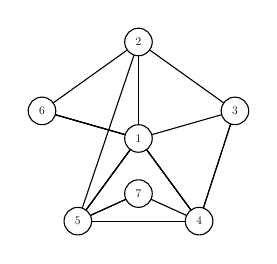
\begin{tikzpicture}[scale=0.35, transform shape, every node/.style={font=\large}]
       
        %add correct 6th here.
       % Define nodes with coordinates
\node[draw, circle, minimum size=1cm] (6) at (0, 0) {$1$};
\node[draw, circle, minimum size=1cm] (4) at (0, -2) {$7$};
\node[draw, circle, minimum size=1cm] (2) at (2.2, -3) {$4$};
\node[draw, circle, minimum size=1cm] (7) at (-3.5, 1) {$6$};
\node[draw, circle, minimum size=1cm] (5) at (3.5, 1) {$3$};
\node[draw, circle, minimum size=1cm] (1) at (0, 3.5) {$2$};
\node[draw, circle, minimum size=1cm] (3) at (-2.2, -3) {$5$};

% Draw edges based on the given connections
\draw[-] (6) -- (1);
\draw[-] (6) -- (2);
\draw[-] (6) -- (3);
\draw[-] (6) -- (7);


\draw[-] (1) -- (3);
\draw[-] (2) -- (3);

\draw[-] (2) -- (5);
\draw[-] (2) -- (6);


\draw[-] (3) -- (4);
\draw[-] (3) -- (6);


\draw[-] (4) -- (2);
\draw[-] (4) -- (3);


\draw[-] (5) -- (1);
\draw[-] (5) -- (2);



\draw[-] (6) -- (1);
\draw[-] (6) -- (2);
\draw[-] (6) -- (3);
\draw[-] (6) -- (5);
\draw[-] (6) -- (7);

\draw[-] (7) -- (1);



\draw[-] (7) -- (6);

        \end{tikzpicture}
    %    \caption{$H_{6}$}
        \label{$H_{6}$}
    }
    
  \vspace{0.6cm} % space between rows
%third row
\subfloat[$H_{7}$]{
        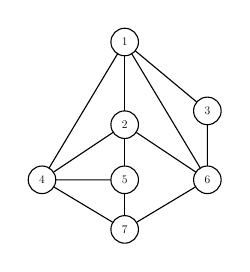
\begin{tikzpicture}[scale=0.35, transform shape, every node/.style={font=\large}]

        %add correct 7th here.
      % Define nodes with coordinates
 % Define nodes with coordinates
\node[draw, circle, minimum size=1cm] (2) at (0, -0.5) {$2$};
\node[draw, circle, minimum size=1cm] (1) at (0, 2.5) {$1$};
\node[draw, circle, minimum size=1cm] (3) at (3, 0) {$3$};
\node[draw, circle, minimum size=1cm] (4) at (-3, -2.5) {$4$};
\node[draw, circle, minimum size=1cm] (5) at (0, -2.5) {$5$};
\node[draw, circle, minimum size=1cm] (6) at (3, -2.5) {$6$};
\node[draw, circle, minimum size=1cm] (7) at (0, -4.3) {$7$};

% Draw edges based on the given connections
\draw[-] (2) -- (1);
\draw[-] (1) -- (3);
\draw[-] (6) -- (1);
\draw[-] (4) -- (1);


\draw[-] (2) -- (4);
\draw[-] (2) -- (6);

\draw[-] (2) -- (5);
\draw[-] (3) -- (6);


\draw[-] (5) -- (4);
\draw[-] (4) -- (7);


\draw[-] (5) -- (7);
\draw[-] (6) -- (7);

        \end{tikzpicture}
       % \caption{$H_{7}$}
        \label{$H_{7}$}
    }
     \hfill
    \subfloat[$H_{8}$]{
        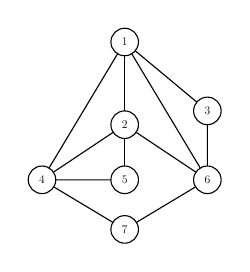
\begin{tikzpicture}[scale=0.35, transform shape, every node/.style={font=\large}]
       
        %add correct 8th here.
       % Define nodes with coordinates
% Define nodes with coordinates
\node[draw, circle, minimum size=1cm] (2) at (0, -0.5) {$2$};
\node[draw, circle, minimum size=1cm] (1) at (0, 2.5) {$1$};
\node[draw, circle, minimum size=1cm] (3) at (3, 0) {$3$};
\node[draw, circle, minimum size=1cm] (4) at (-3, -2.5) {$4$};
\node[draw, circle, minimum size=1cm] (5) at (0, -2.5) {$5$};
\node[draw, circle, minimum size=1cm] (6) at (3, -2.5) {$6$};
\node[draw, circle, minimum size=1cm] (7) at (0, -4.3) {$7$};

% Draw edges based on the given connections
\draw[-] (2) -- (1);
\draw[-] (1) -- (3);
\draw[-] (6) -- (1);
\draw[-] (4) -- (1);


\draw[-] (2) -- (4);
\draw[-] (2) -- (6);

\draw[-] (2) -- (5);
\draw[-] (3) -- (6);


\draw[-] (5) -- (4);
\draw[-] (4) -- (7);



\draw[-] (6) -- (7);

\end{tikzpicture}
  %   \caption{$H_{8}$}
     \label{$H_{8}$}
}
\hfill
\subfloat[$H_{9}$]{
        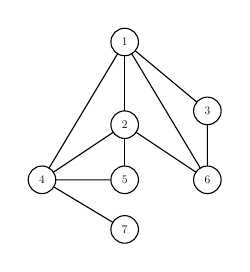
\begin{tikzpicture}[scale=0.35, transform shape, every node/.style={font=\large}]

        %add correct 9th here.
      % Define nodes with coordinates
 % Define nodes with coordinates
% Define nodes with coordinates
\node[draw, circle, minimum size=1cm] (2) at (0, -0.5) {$2$};
\node[draw, circle, minimum size=1cm] (1) at (0, 2.5) {$1$};
\node[draw, circle, minimum size=1cm] (3) at (3, 0) {$3$};
\node[draw, circle, minimum size=1cm] (4) at (-3, -2.5) {$4$};
\node[draw, circle, minimum size=1cm] (5) at (0, -2.5) {$5$};
\node[draw, circle, minimum size=1cm] (6) at (3, -2.5) {$6$};
\node[draw, circle, minimum size=1cm] (7) at (0, -4.3) {$7$};

% Draw edges based on the given connections
\draw[-] (2) -- (1);
\draw[-] (1) -- (3);
\draw[-] (6) -- (1);
\draw[-] (4) -- (1);


\draw[-] (2) -- (4);
\draw[-] (2) -- (6);

\draw[-] (2) -- (5);
\draw[-] (3) -- (6);


\draw[-] (5) -- (4);
\draw[-] (4) -- (7);

     \end{tikzpicture}
      %  \caption{$H_{9}$}
         \label{$H_{9}$}
    }
    
      \vspace{0.6cm} % space between rows
      %fourth row.
    \subfloat[$H_{10}$]{
        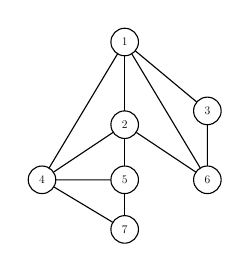
\begin{tikzpicture}[scale=0.35, transform shape, every node/.style={font=\large}]
       
        %add correct 10th here.
       % Define nodes with coordinates
% Define nodes with coordinates

% Define nodes with coordinates
\node[draw, circle, minimum size=1cm] (2) at (0, -0.5) {$2$};
\node[draw, circle, minimum size=1cm] (1) at (0, 2.5) {$1$};
\node[draw, circle, minimum size=1cm] (3) at (3, 0) {$3$};
\node[draw, circle, minimum size=1cm] (4) at (-3, -2.5) {$4$};
\node[draw, circle, minimum size=1cm] (5) at (0, -2.5) {$5$};
\node[draw, circle, minimum size=1cm] (6) at (3, -2.5) {$6$};
\node[draw, circle, minimum size=1cm] (7) at (0, -4.3) {$7$};

% Draw edges based on the given connections
\draw[-] (2) -- (1);
\draw[-] (1) -- (3);
\draw[-] (6) -- (1);
\draw[-] (4) -- (1);


\draw[-] (2) -- (4);
\draw[-] (2) -- (6);

\draw[-] (2) -- (5);
\draw[-] (3) -- (6);


\draw[-] (5) -- (4);
\draw[-] (4) -- (7);


\draw[-] (5) -- (7);

        \end{tikzpicture}
      %  \caption{$H_{10}$}
         \label{$H_{10}$}
    } 
     \hfill
  \subfloat[$H_{11}$]{
 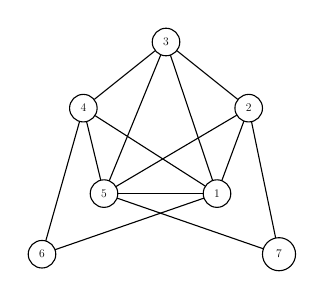
\begin{tikzpicture}[scale=0.35, transform shape, every node/.style={font=\large}]
\node[draw, text=black, circle, minimum size=1cm] (1) at (1.15, -2.5) {$1$};

\node[draw, circle, minimum size=1cm] (2) at (2.3, 0.6) {$2$};

\node[draw, circle, minimum size=1cm] (4) at (-3.7, 0.6) {$4$};

\node[draw, circle, minimum size=1cm] (3) at (-0.7, 3) {$3$};

\node[draw, circle, minimum size=1cm] (5) at (-2.95, -2.5) {$5$};

\node[draw, circle, minimum size=1cm] (6) at (-5.2, -4.7) {$6$};

\node[draw, circle, minimum size=1.2cm] (7) at (3.4, -4.7) {$7$};

\draw[-] (1) -- (2);
\draw[-] (2) -- (3);
\draw[-] (3) -- (4);

\draw[-] (1) -- (5);
\draw[-] (1) -- (3);
\draw[-] (5) -- (4);

\draw[-] (5) -- (2);
\draw[-] (5) -- (3);
\draw[-] (1) -- (4);

\draw[-] (1) -- (6);
\draw[-] (4) -- (6);

\draw[-] (2) -- (7);
\draw[-] (5) -- (7);

 \end{tikzpicture}
%\caption{$H_{11}$}
 \label{$H_{11}$}
  }
    \caption{Minimal non-comparability graphs - $4$}
    \label{fig:min-non-comp-part4}
\end{figure}

In the following section, we identify all the minimal non-comparability graphs that are semi-transitive. 


\section{Minimal non-comparability graphs that are semi-transitive}
\label{section-min-semi-trans}
In this section, we prove that several minimal non-comparability graphs are semi-transitive. Theorem \ref{3-color-graphs-theorem} shows that three of the infinite classes of minimal non-comparability graphs are $3$-colorable and hence word-representable.


\begin{theorem}
\label{3-color-graphs-theorem}
    The graph classes $G_{n}^{1}$, $G_{n}^{2}$, and $G_{n}^{3}$ shown in Figure \ref{fig:min-non-comp-part1} constitute a subclass of $3$-colorable graphs.
\end{theorem}


\begin{proof}
For any graph \( G \in G_{n}^{1} \), the vertex set can be partitioned into three independent sets: \( A \), \( B \), and \( C \), where 
$A = \{1,3, \ldots, 2n-1\}$,  $B = \{2,4, \ldots, 2n\}$, and $C = \{2n+1\}$. Similarly, any graph \( G \in G_{n}^{2} \) can be vertex partitioned into three independent sets: \( A \), \( B \), and \( C \), where $A = \{1, x, y\}$, $B = \{2,4,6, \ldots, 2n\}$, and $C = \{3,5,7, \ldots, 2n+1\}$. Likewise, for any graph \( G \in G_{n}^{3} \), the vertex set can be partitioned into three independent sets: \( A \), \( B \), and \( C \), with 
$A = \{1, 2n\}$, $B = \{2,4,6, \ldots, 2n-2, x\}$, and $C = \{3,5,7, \ldots, 2n-1, y\}$.
Figure \ref{fig:3-colo-graphs} demonstrates the $3$-colorability of these graph classes.


\begin{figure}[h]
    \centering
    \subfloat[$G_{n}^{1}$]{
%for cycle 2n+1.
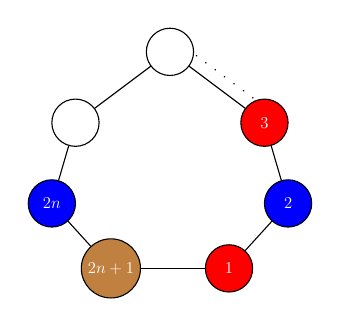
\begin{tikzpicture}[scale=0.5, transform shape, every node/.style={font=\large}]

\node[draw, circle, fill=red, text=white, minimum size=1.2cm] (1) at (2, 0) {$1$};
\node[draw, circle, fill=blue, text=white, minimum size=1.2cm] (2) at (3.5, 1.65) {$2$};
\node[draw, circle, fill=red, text=white, minimum size=1.2cm] (3) at (2.9, 3.7) {$3$};
\node[draw, circle, fill=white, minimum size=1.2cm] (r) at (0.5, 5.5) {};
\node[draw, circle, fill=white, minimum size=1.2cm] (r1) at (-1.9, 3.7) {};
\node[draw, circle, fill=blue, text=white, minimum size=1.2cm] (2n) at (-2.5, 1.65) {$2n$};
\node[draw, circle, fill=brown, text=white, minimum size=1.2cm] (2n+1) at (-1, 0) {$2n+1$};

\draw[-] (1) -- (2);
\draw[-] (2) -- (3);
\draw[-] (3) -- (r) node[midway, sloped, above, yshift=5pt] {. . . . . . .}; % Label shifted a bit upward
\draw[-] (r) -- (r1);
\draw[-] (r1) -- (2n);
\draw[-] (2n) -- (2n+1);
\draw[-] (2n+1) -- (1);

\end{tikzpicture}

%\caption{$G_{n}^{1}$}
\label{fig:3-colo-g1n}
}
\hfill
\subfloat[$G_{n}^{2}$]{
        % Second TikZ picture
 
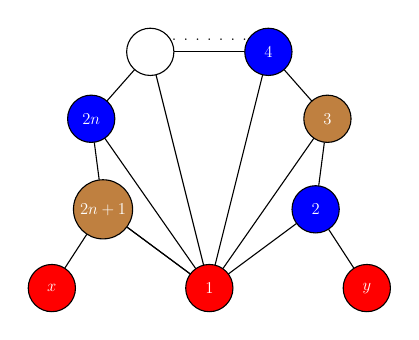
\begin{tikzpicture}[scale=0.5, transform shape, every node/.style={font=\large}]

\node[draw, circle, fill=red, text=white, minimum size=1.2cm] (1) at (0, -2) {$1$};
\node[draw, circle, fill=blue, text=white, minimum size=1.2cm] (2) at (2.7, 0) {$2$};
\node[draw, circle, fill=brown, text=white, minimum size=1.2cm] (2n+1) at (-2.7, 0) {$2n+1$};
\node[draw, circle, fill=brown, text=white, minimum size=1.2cm] (3) at (3, 2.3) {$3$};
\node[draw, circle, fill=blue, text=white, minimum size=1.2cm] (4) at (1.5, 4) {$4$};
\node[draw, circle, fill=white, minimum size=1.2cm] (r) at (-1.5, 4) {};
\node[draw, circle, fill=blue, text=white, minimum size=1.2cm] (2n) at (-3, 2.3) {$2n$};
\node[draw, circle, fill=red, text=white, minimum size=1.2cm] (x) at (-4, -2) {$x$};
\node[draw, circle, fill=red, text=white, minimum size=1.2cm] (y) at (4, -2) {$y$};

\draw[-] (1) -- (2);
\draw[-] (2) -- (3);
\draw[-] (3) -- (4);
\draw[-] (4) -- (r) node[midway, above, yshift=5pt] {. . . . . . .};
\draw[-] (r) -- (2n);
\draw[-] (2n) -- (2n+1);
\draw[-] (2n+1) -- (1);
\draw[-] (1) -- (3);
\draw[-] (1) -- (4);
\draw[-] (1) -- (r);
\draw[-] (1) -- (2n);
\draw[-] (1) -- (2n+1);
\draw[-] (2n+1) -- (x);
\draw[-] (2) -- (y);

\end{tikzpicture}

% \caption{$G_{n}^{2}$}
\label{fig:3-colo-g2n}
}
      \hfill
\subfloat[$G_{n}^{3}$]{
        % Third TikZ picture
     
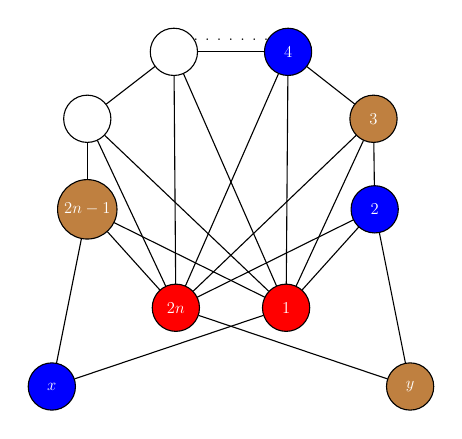
\begin{tikzpicture}[scale=0.5, transform shape, every node/.style={font=\large}]

\node[draw, circle, fill=red, text=white, minimum size=1.2cm] (1) at (1.15, -2.5) {$1$};
\node[draw, circle, fill=blue, text=white, minimum size=1.2cm] (2) at (3.4, 0) {$2$};
\node[draw, circle, fill=brown, text=white, minimum size=1.2cm] (2n-1) at (-3.9, 0) {$2n-1$};
\node[draw, circle, fill=brown, text=white, minimum size=1.2cm] (3) at (3.37, 2.3) {$3$};
\node[draw, circle, fill=white, minimum size=1.2cm] (r1) at (-3.9, 2.3) {};
\node[draw, circle, fill=blue, text=white, minimum size=1.2cm] (4) at (1.2, 4) {$4$};
\node[draw, circle, fill=white, minimum size=1.2cm] (r) at (-1.7, 4) {};
\node[draw, circle, fill=red, text=white, minimum size=1.2cm] (2n) at (-1.65, -2.5) {$2n$};
\node[draw, circle, fill=blue, text=white, minimum size=1.2cm] (x) at (-4.8, -4.5) {$x$};
\node[draw, circle, fill=brown, text=white, minimum size=1.2cm] (y) at (4.3, -4.5) {$y$};

\draw[-] (1) -- (2);
\draw[-] (2) -- (3);
\draw[-] (3) -- (4);
\draw[-] (4) -- (r) node[midway, above, yshift=5pt] {. . . . . . .};
\draw[-] (1) -- (3);
\draw[-] (1) -- (4);
\draw[-] (1) -- (r);
\draw[-] (1) -- (r1);
\draw[-] (1) -- (2n-1);
\draw[-] (2n) -- (2);
\draw[-] (2n) -- (3);
\draw[-] (2n) -- (4);
\draw[-] (2n) -- (r);
\draw[-] (2n) -- (r1);
\draw[-] (2n) -- (2n-1);
\draw[-] (r) -- (r1);
\draw[-] (2n-1) -- (r1);
\draw[-] (2n-1) -- (x);
\draw[-] (2) -- (y);
\draw[-] (2n) -- (y);
\draw[-] (1) -- (x);

\end{tikzpicture}

%\caption{$G_{n}^{3}$}
\label{fig:3-colo-g3n}
}
\caption{$3$-colorable minimal non-comparability graph classes}
\label{fig:3-colo-graphs}
\end{figure}


\end{proof}

From Theorem \ref{3-color-graphs-theorem} and Theorem \ref{3-col_is_semi}, we have the following Corollary \ref{g123word-rep-cor}.
\begin{corollary}
\label{g123word-rep-cor}
    The class of graphs $G_{n}^{1}, G_{n}^{2}$, and $G_{n}^{3}$ form a subclass of word-representable graphs.
\end{corollary}

\begin{theorem}
    The class of graphs $G_{n}^{5}$ depicted in Figure \ref{g5n} form a subclass of word-representable graphs.
\end{theorem}

\begin{proof}
    Consider an arbitrary graph $G \in G_{n}^{5}$, where $|V(G)|=2n$ and $|E(G)|=\binom{2n}{2} - 2n$. The $2n$ edges, which are absent in $G$, form a cycle as shown in Figure \ref{fig:min-non-comp-part2}. Let $A$ denote the set $\{a_{1}, a_{2}, \cdots a_{n}\}$  and $B$ denote the set $\{b_{1}, b_{2}, \cdots b_{n}\}$. Note that each of the sets $A$ and $B$ induce a clique in $G$. We provide a semi-transitive orientation of $G$. Consider the following orientation for edges in $G$. An edge between two vertices in $G$ is oriented from the vertex with a smaller index value to the vertex with a larger index value. This is shown in Figure \ref{fig:orientationofg5n}. This orientation is acyclic. For the sake of contradiction, assume that the orientation provided in Figure \ref{fig:orientationofg5n} is not semi-transitive. That implies that at least one directed path exists that violates semi-transitivity. Consider a path $P= u_{1} \rightarrow u_{2} \rightarrow \cdots \rightarrow u_{k}$ that violates semi-transitivity, where $u_{r}$ is either $a_{i}$ or $b_{j}$. The edge $u_{1} \rightarrow u_{k}$ is present and some edge $\{u_{i}, u_{j}\}$ is missing, where $1 \leq i < j \leq k$. 
    \begin{note}
    \label{note:g5-path-increasing}
        Any directed path in $G$ under the orientation provided in Figure \ref{fig:orientationofg5n} has the index of vertices in strictly increasing order.
    \end{note}
    The missing edges in $G$ can be categorized into two types.
    \begin{enumerate}
        \item Type $1: \{a_{i}, b_{j}\}$,  where $|i-j| \leq 1$.
        \item Type $2:  \{a_{1}, b_{n}\}$
    \end{enumerate}
 If the missing edge $\{u_{i}, u_{j}\}$ in the path $P$ is a Type $1$ edge, then from Note \ref{note:g5-path-increasing}, it can only be the adjacent vertices in $P$. That's a contradiction, and hence the missing edge $\{u_{i}, u_{j}\}$ in the path $P$ cannot be a Type $1$ edge.  Hence, $\{u_{i}, u_{j}\}$ can only be $\{a_{1}, b_{n}\}$. Due to the specific orientation of edges in the graph $G$, if $a_1$ and $b_n$ are present in the path $P$, then $a_1$ must be the starting vertex, and $b_n$ must be the ending vertex. That is, $u_1 = a_1$ and $u_k = b_n$. However, since $u_1$ is not connected to $u_k$, this leads to a contradiction. Therefore, our initial assumption is false, confirming that the orientation is semi-transitive.

\begin{figure}[h]
    \centering
\subfloat[When $j>i$]{
\centering
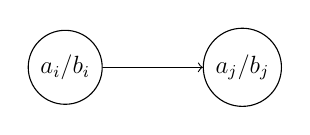
\begin{tikzpicture}[scale=0.75, transform shape, every node/.style={font=\large}]

\node[draw, circle,  minimum size=1.2cm] (1) at (0, 0) {$a_{i}/b_{i}$};
\node[draw, circle,  minimum size=1.2cm] (2) at (3, 0) {$a_{j}/b_{j}$};

\draw[->] (1) -- (2);

\end{tikzpicture}
%\caption{When $j > i$}
\label{fig:j>i}
     }
     \hfill
    \subfloat[When $i>j$]{
\centering
         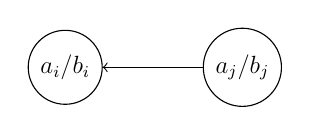
\begin{tikzpicture}[scale=0.75, transform shape, every node/.style={font=\large}]

\node[draw, circle,  minimum size=1.2cm] (1) at (0, 0) {$a_{i}/b_{i}$};
\node[draw, circle,  minimum size=1.2cm] (2) at (3, 0) {$a_{j}/b_{j}$};
\draw[->] (2) -- (1);
\end{tikzpicture}
%\caption{When $i >j$}
\label{fig:i>j}
}
\caption{A semi-transitive orientation of edges of $G \in G_{n}^{5}$ }
\label{fig:orientationofg5n}
\end{figure}


\end{proof}


\begin{theorem}
    The class of graphs $G_{n}^{6}$ depicted in Figure \ref{g6n} form a subclass of word-representable graphs.
\end{theorem}



\begin{proof}
    Consider an arbitrary graph $G \in G_{n}^{6}$, where $|V(G)|=2n+1$ and $|E(G)|=\binom{2n+1}{2} - (2n+1)$. The $2n+1$ edges, which are absent in $G$, form a cycle as shown in Figure \ref{fig:min-non-comp-part2}. Let $A$ denote the set $\{a_{1}, a_{2}, \cdots a_{n}\}$  and $B$ denote the set $\{b_{1}, b_{2}, \cdots b_{n}\}$. Note that each of the sets $A$ and $B$ induce a clique in $G$. We provide a semi-transitive orientation of $G$. Consider the following orientation for edges in $G$. An edge between two vertices in $G$ is oriented from the vertex with a smaller index value to the vertex with a larger index value. This is shown in Figure \ref{fig:orientationofg6n}. This orientation is acyclic. For the sake of contradiction, assume that the orientation provided in Figure \ref{fig:orientationofg6n} is not semi-transitive. That implies that at least one directed path exists that violates semi-transitivity. Consider a path $P= u_{1} \rightarrow u_{2} \rightarrow \cdots \rightarrow u_{k}$ that violates semi-transitivity, where $u_{r}$ is either $a_{i}$ or $b_{j}$. The edge $u_{1} \rightarrow u_{k}$ is present and some edge $\{u_{i}, u_{j}\}$ is missing, where $1 \leq i < j \leq k$. 
    \begin{note}
    \label{note:g6-path-increasing}
        Any directed path in $G$ under the orientation provided in Figure \ref{fig:orientationofg6n} has the index of vertices in strictly increasing order.
    \end{note}
    The missing edges in $G$ can be categorized into two types.
   \begin{enumerate}
        \item Type $1: \{a_{i}, b_{j}\}$ in $G$, where $|i-j| \leq 1$.
        \item Type $2:  \{c_{0}, b_{n}\}$
    \end{enumerate}
        If the missing edge $\{u_{i}, u_{j}\}$ in the path $P$ is a Type $1$ edge, then from Note \ref{note:g6-path-increasing}, it can only be the adjacent vertices in $P$. That's a contradiction, and hence the missing edge $\{u_{i}, u_{j}\}$ in the path $P$ cannot be a Type $1$ edge.  Hence, $\{u_{i}, u_{j}\}$ can only be $\{c_{0}, b_{n}\}$. Due to the specific orientation of edges in the graph $G$, if $c_{0}$ and $b_{n}$ are present in the path $P$, then $c_0$ must be the starting vertex, and $b_n$ must be the ending vertex. That is, $u_1 = c_0$ and $u_k = b_n$. However, since $u_1$ is not connected to $u_k$, this leads to a contradiction. Therefore, our initial assumption is false, confirming that the orientation is semi-transitive.

\begin{figure}[h]
    \centering
\subfloat[When $j>i$]{
\centering
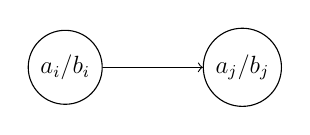
\begin{tikzpicture}[scale=0.75, transform shape, every node/.style={font=\large}]

\node[draw, circle,  minimum size=1.2cm] (1) at (0, 0) {$a_{i}/b_{i}$};
\node[draw, circle,  minimum size=1.2cm] (2) at (3, 0) {$a_{j}/b_{j}$};

\draw[->] (1) -- (2);

\end{tikzpicture}
%\caption{When $j > i$}
\label{fig:j>i(g6n)}
     }
     \hfill
     \subfloat[When $i>j$]{
\centering
         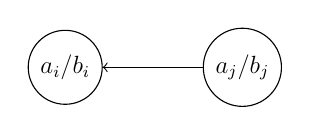
\begin{tikzpicture}[scale=0.75, transform shape, every node/.style={font=\large}]

\node[draw, circle,  minimum size=1.2cm] (1) at (0, 0) {$a_{i}/b_{i}$};
\node[draw, circle,  minimum size=1.2cm] (2) at (3, 0) {$a_{j}/b_{j}$};
\draw[->] (2) -- (1);
\end{tikzpicture}
%\caption{When $i >j$}
\label{fig:i>j(g6n)}
}
\hfill
\subfloat[$c_{0}$ as a source vertex]{
\centering
         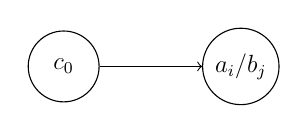
\begin{tikzpicture}[scale=0.75, transform shape, every node/.style={font=\large}]

\node[draw, circle,  minimum size=1.2cm] (1) at (0, 0) {$c_{0}$};
\node[draw, circle,  minimum size=1.2cm] (2) at (3, 0) {$a_{i}/b_{j}$};
\draw[->] (1) -- (2);
\end{tikzpicture}
%\caption{$c_{0}$ as a source vertex}
\label{fig:c0source}
}
\caption{A semi-transitive orientation of edges of $G \in G_{n}^{6}$}
\label{fig:orientationofg6n}
\end{figure}


\end{proof}



\begin{theorem}
\label{theorem-g7n}
    The class of graphs $G_{n}^{7}$ depicted in Figure \ref{g7n} form a subclass of word-representable graphs.
\end{theorem}

\begin{proof}


Consider an arbitrary graph \( G \in G_{n}^{7} \). As illustrated in Figure \ref{g7n}, the graph is structured into three levels. The vertex sets corresponding to levels $1, 2$, and $3$ are \( \{a, b, c, d\} \), \( \{1, 2, \dots, n\} \), and \( \{x\} \), respectively. Consider the orientation of the edges of $G$ as shown in Figure \ref{fig:orientationofg7n}. This orientation is acyclic.  We show that this is a semi-transitive orientation of $G$ by showing that none of the paths in $G$ violate semi-transitivity.  In Figure \ref{fig:acrosslevel-orient-g7n}, $L1, L2$ and $L3$ denote any vertex from Level $1$, Level $2$ and Level $3$ respectively.

\begin{figure}[h]
    \centering
\subfloat[Orientation of edges in Level $1$.]{
\centering
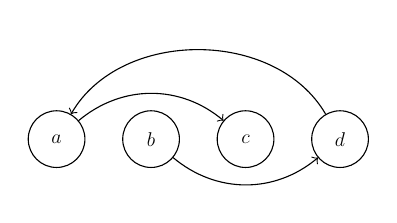
\begin{tikzpicture}[scale=0.6, transform shape, every node/.style={font=\large}]

\node[draw, circle,  minimum size=1.2cm] (1) at (-1, 0) {$a$};
\node[draw, circle,  minimum size=1.2cm] (2) at (1, 0) {$b$};
\node[draw, circle,  minimum size=1.2cm] (3) at (3, 0) {$c$};
\node[draw, circle,  minimum size=1.2cm] (4) at (5, 0) {$d$};

 % Draw edges with curved paths
    \draw[->, bend left=40] (1) to (3);  % Curves up
    \draw[->, bend right=40] (2) to (4); % Curves down
    \draw[->, bend right=60] (4) to (1);  % Ensure it curves up


\end{tikzpicture}
%\caption{Orientation of edges in Level $1$.}
\label{fig:level-1orient-g7n}
    }
     \hfill
   \subfloat[Orientation of edges in Level $2$.]{
\centering

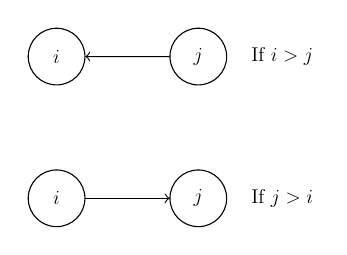
\begin{tikzpicture}[scale=0.6, transform shape, every node/.style={font=\large}]

\node[draw, circle,  minimum size=1.2cm] (1) at (0, 0) {$i$};
\node[draw, circle,  minimum size=1.2cm] (2) at (3, 0) {$j$};
\node[draw, circle,  minimum size=1.2cm] (3) at (0, 3) {$i$};
\node[draw, circle,  minimum size=1.2cm] (4) at (3, 3) {$j$};

\draw[->] (1) -- (2);
\draw[->] (4) -- (3);

% Add text near vertices
    \node[right, xshift= 1cm] at (2) {If $j > i$};
    \node[right, xshift= 1cm] at (4) {If $i>j$};
    
\end{tikzpicture}
%\caption{Orientation of edges in Level $2$.}
\label{fig:level-orient-2-g7n}
}
\hfill
\subfloat[Orientation of edges across levels.]{
\centering
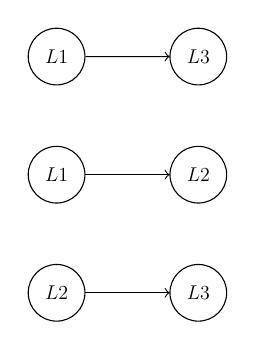
\begin{tikzpicture}[scale=0.6, transform shape, every node/.style={font=\large}]

\node[draw, circle,  minimum size=1.2cm] (1) at (0, 0) {$L1$};
\node[draw, circle,  minimum size=1.2cm] (2) at (3, 0) {$L2$};
\node[draw, circle,  minimum size=1.2cm] (3) at (3, 2.5) {$L3$};
\node[draw, circle,  minimum size=1.2cm] (4) at (0, 2.5) {$L1$};
\node[draw, circle,  minimum size=1.2cm] (5) at (0, -2.5) {$L2$};
\node[draw, circle,  minimum size=1.2cm] (6) at (3, -2.5) {$L3$};


\draw[->] (1) -- (2);
\draw[->] (4) -- (3);
\draw[->] (5) -- (6);

\end{tikzpicture}
%\caption{Orientation of edges across levels. $($$L1, L2$ and $L3$ denote any vertex from Level $1$, Level $2$ and Level $3$ respectively.$)$}
\label{fig:acrosslevel-orient-g7n}
}
\caption{A semi-transitive orientation of edges of $G \in G_{n}^{7}$.}
\label{fig:orientationofg7n}
\end{figure}

\begin{note}
    No path originates from a level $2$ vertex and terminates at a level $1$ vertex. Similarly, no path starts at level $3$ and ends at any other level.
\end{note}

    \begin{lemma}
    \label{level2}
        Consider $G$ with its orientation as shown in Figure \ref{fig:orientationofg7n}. Any path that starts and ends at a level $2$ vertex does not violate the semi-transitivity property.
    \end{lemma}
    
    \begin{proof}
    Consider an arbitrary path $P= u_{1} \rightarrow u_{2} \rightarrow \cdots \rightarrow u_{k}$, where each vertex $u_{i}$, for $1 \leq i \leq k$, belongs to level $2$. For any consecutive vertices $u_{i}$ and $u_{j}$ in $P$, we have $|u_{i}-u_{j}| \geq 2$. Suppose $P$ violates semi-transitivity. This implies that the edge $u_{1} \rightarrow u_{k}$ is present, but some edge $\{u_{i}, u_{j}\}$ is missing for some $1 \leq i < j \leq k$. Since the only missing edges in level $2$ are of the form $\{i, i+1\}$ for $1 \leq i \leq (n-1)$, this leads to a contradiction. Hence, our assumption is false, confirming that $P$ does not violate semi-transitivity.
    \end{proof}
    
    \begin{observation}
        \label{level1}
        Consider $G$ with its orientation as shown in Figure \ref{fig:orientationofg7n}. Any path that starts and ends at a level $1$ vertex does not violate the semi-transitivity property.
    \end{observation}

    \begin{proof}
    The longest path within level $1$ has a length of $3$, given by $P = b \rightarrow d \rightarrow a \rightarrow c$. The path $P$ does not violate semi-transitivity, as the edge $b \rightarrow c$ is absent. Additionally, any path with a length of at most $2$ does not violate semi-transitivity.

    \end{proof}

    \begin{lemma}
    \label{level1to2}
        Consider the graph \( G \) with its orientation as depicted in Figure \ref{fig:orientationofg7n}. Any path in \( G \) that begins at a level 1 vertex and terminates at a level 2 vertex adheres to the semi-transitivity property.
    \end{lemma}
    
    \begin{proof}
        The only vertices in level $1$ that are adjacent to vertices in level $2$ are \( d \) and \( a \). Therefore, it suffices to demonstrate that the paths starting at \( a \) or \( d \) do not violate the semi-transitivity property. Consider an arbitrary path \( P \) that begins at vertex \( a \) and terminates at a vertex in level $2$. For \( P \) to end at a level $2$ vertex, its neighboring vertex must be from level $2$. Vertex \( a \) is connected to all vertices in level $2$, except for vertex $1$. Therefore, if \( a \) is the starting vertex of path \( P \), vertex $1$ cannot appear in \( P \). Since \( a \) is connected to every vertex in level $2$, and by Lemma \ref{level2}, we conclude that \( P \) does not violate the semi-transitivity property. Consider an arbitrary path \( P \) that begins at vertex \( d \) and terminates at a vertex in level \( 2 \). The path \( P \) can be of two types:
\begin{enumerate}
    \item Type \( 1 \): \( d \rightarrow a \rightarrow \) level \( 2 \) vertices.
    \item Type \( 2 \): \( d \rightarrow \) level \( 2 \) vertices.
\end{enumerate}
Consider \( P \) of Type \( 2 \). Vertex \( d \) is adjacent to all vertices in level \( 2 \), except \( n \). If \( n \) appears in \( P \), it must be at the end. By Lemma \ref{level2}, \( P \) does not violate the semi-transitivity property.  For \( P \) of Type \( 1 \), a similar argument applies. Paths of the form \( a \rightarrow \) level \( 2 \) vertices satisfy semi-transitivity. Prepending \( d \) does not violate this property, as \( d \) is adjacent to all level \( 2 \) vertices except \( n \). If \( n \) appears in \( P \), it must be at the end. By Lemma \ref{level2}, \( P \) does not violate semi-transitivity.

    \end{proof}

\begin{observation}
    Consider \( G \) with its orientation as shown in Figure \ref{fig:orientationofg7n}. Any path in \( G \) that terminates at a level \( 3 \) vertex preserves the semi-transitivity property.
\end{observation}

\begin{proof}
    The vertex \( x \) is adjacent to all vertices except \( b \) and \( c \). However, \( b \) and \( c \) (both in level \( 1 \)) are not connected to any vertices from other levels. Therefore, by Observation \ref{level1}, Lemma \ref{level2}, and Lemma \ref{level1to2}, any path in \( G \) ending at \( x \) maintains semi-transitivity.
\end{proof}

    

\end{proof}

\begin{theorem}
\label{theorem-g8n}
    The class of graphs $G_{n}^{8}$ depicted in Figure \ref{g8n} form a subclass of word-representable graphs.
\end{theorem}

The proof of Theorem \ref{theorem-g8n} follows the same approach as the proof of Theorem \ref{theorem-g7n}. Although the orientation in level \( 1 \) differs slightly, it does not affect the validity of the proof. A semi-transitive orientation of the edges in an arbitrary graph \( G \in G_{n}^{8} \) is shown in Figure \ref{fig:orientationofg8n}.


\begin{figure}[h]
    \centering
\subfloat[Orientation of edges in Level $1$.]{
\centering
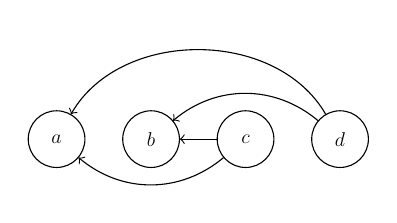
\begin{tikzpicture}[scale=0.6, transform shape, every node/.style={font=\large}]

\node[draw, circle,  minimum size=1.2cm] (1) at (-1, 0) {$a$};
\node[draw, circle,  minimum size=1.2cm] (2) at (1, 0) {$b$};
\node[draw, circle,  minimum size=1.2cm] (3) at (3, 0) {$c$};
\node[draw, circle,  minimum size=1.2cm] (4) at (5, 0) {$d$};

 % Draw edges with curved paths
    \draw[->, bend left=40] (3) to (1);  % Curves up
    \draw[->, bend right=40] (4) to (2); % Curves down
    \draw[->, bend right=60] (4) to (1);  % Ensure it curves up
\draw[->] (3) to (2);

\end{tikzpicture}
%\caption{Orientation of edges in Level $1$.}
\label{fig:level-1orient-g8n}
    }
     \hfill
    \subfloat[Orientation of edges in Level $2$.]{
\centering

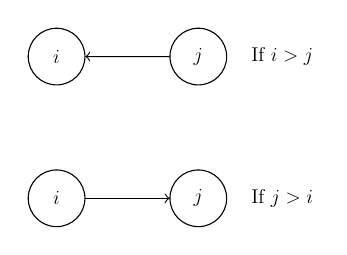
\begin{tikzpicture}[scale=0.6, transform shape, every node/.style={font=\large}]

\node[draw, circle,  minimum size=1.2cm] (1) at (0, 0) {$i$};
\node[draw, circle,  minimum size=1.2cm] (2) at (3, 0) {$j$};
\node[draw, circle,  minimum size=1.2cm] (3) at (0, 3) {$i$};
\node[draw, circle,  minimum size=1.2cm] (4) at (3, 3) {$j$};

\draw[->] (1) -- (2);
\draw[->] (4) -- (3);

% Add text near vertices
    \node[right, xshift= 1cm] at (2) {If $j > i$};
    \node[right, xshift= 1cm] at (4) {If $i>j$};
    
\end{tikzpicture}
%\caption{Orientation of edges in Level $2$.}
\label{fig:level-orient-2-g8n}
}
\hfill
\subfloat[Orientation of edges across levels.]{
\centering
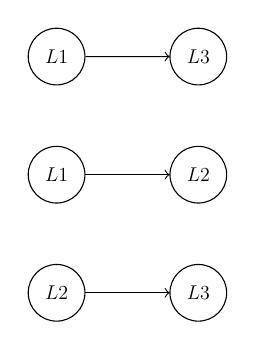
\begin{tikzpicture}[scale=0.6, transform shape, every node/.style={font=\large}]

\node[draw, circle,  minimum size=1.2cm] (1) at (0, 0) {$L1$};
\node[draw, circle,  minimum size=1.2cm] (2) at (3, 0) {$L2$};
\node[draw, circle,  minimum size=1.2cm] (3) at (3, 2.5) {$L3$};
\node[draw, circle,  minimum size=1.2cm] (4) at (0, 2.5) {$L1$};
\node[draw, circle,  minimum size=1.2cm] (5) at (0, -2.5) {$L2$};
\node[draw, circle,  minimum size=1.2cm] (6) at (3, -2.5) {$L3$};


\draw[->] (1) -- (2);
\draw[->] (4) -- (3);
\draw[->] (5) -- (6);

\end{tikzpicture}
%\caption{Orientation of edges across levels. $($$L1, L2$ and $L3$ denote any vertex from Level $1$, Level $2$ and Level $3$ respectively.$)$}
\label{fig:acrosslevel-orient-g8n}
}
\caption{A semi-transitive orientation of edges of $G \in G_{n}^{8}$.}
\label{fig:orientationofg8n}
\end{figure}

\begin{remark}
\label{remark-semi-graphs}
    The graphs identified as semi-transitive from the set of minimal comparability graphs depicted in Figure \ref{fig:min-non-comp-part4} are presented along with their corresponding semi-transitive orientations in Figure \ref{fig:min-non-comp-part4-semi-trans}. Since these graphs are relatively small and can be individually verified as semi-transitive through straightforward inspection, we omit formal proofs.
\end{remark}
\begin{figure}[htbp]
    \centering
    % First row
    \subfloat[$H_{2}$]{
        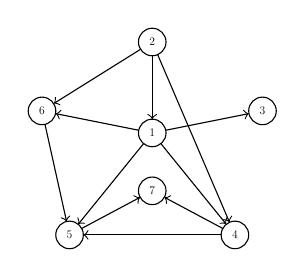
\begin{tikzpicture}[scale=0.35, transform shape, every node/.style={font=\large}]
        % Define nodes with coordinates
        \node[draw, circle, minimum size=1cm] (7) at (0, 0.2) {$1$};
        \node[draw, circle, minimum size=1cm] (4) at (0, -1.9) {$7$};
        \node[draw, circle, minimum size=1cm] (2) at (3, -3.5) {$4$};
        \node[draw, circle, minimum size=1cm] (3) at (-4, 1) {$6$};
        \node[draw, circle, minimum size=1cm] (1) at (4, 1) {$3$};
        \node[draw, circle, minimum size=1cm] (5) at (0, 3.5) {$2$};
        \node[draw, circle, minimum size=1cm] (6) at (-3, -3.5) {$5$};

        % Draw edges based on the given connections
        \draw[->] (7) -- (3);
        \draw[->] (7) -- (1);
        \draw[<-] (7) -- (5);
        \draw[->] (7) -- (6);
        \draw[->] (7) -- (2);
        \draw[<-] (2) -- (5);
        \draw[->] (2) -- (6);
        \draw[<-] (3) -- (5);
        \draw[->] (3) -- (6);
        \draw[<-] (4) -- (2);
        \draw[<-] (4) -- (6);
        \end{tikzpicture}
     %   \caption{$H_{2}$}
       
    }
    \hfill
    \subfloat[$H_{3}$]{
        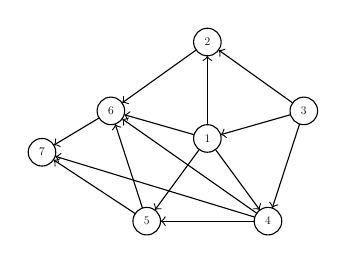
\begin{tikzpicture}[scale=0.35, transform shape, every node/.style={font=\large}]
        % Define nodes with coordinates
        \node[draw, circle, minimum size=1cm] (1) at (0, 0) {$1$};
        \node[draw, circle, minimum size=1cm] (2) at (-6, -0.5) {$7$};
        \node[draw, circle, minimum size=1cm] (6) at (2.2, -3) {$4$};
        \node[draw, circle, minimum size=1cm] (7) at (-3.5, 1) {$6$};
        \node[draw, circle, minimum size=1cm] (5) at (3.5, 1) {$3$};
        \node[draw, circle, minimum size=1cm] (3) at (0, 3.5) {$2$};
        \node[draw, circle, minimum size=1cm] (4) at (-2.2, -3) {$5$};

        % Draw edges based on the given connections
        \draw[->] (1) -- (3);
        \draw[->] (1) -- (4);
        \draw[<-] (1) -- (5);
        \draw[->] (1) -- (6);
        \draw[->] (1) -- (7);
  


        \draw[<-] (3) -- (5);
        \draw[->] (3) -- (7);
 
        \draw[->] (4) -- (2);
      
        \draw[->] (5) -- (6);
    
        \draw[->] (6) -- (2);
        \draw[->] (6) -- (4);
      
        \draw[->] (7) -- (2);
  
        \draw[<-] (7) -- (4);
        \draw[<-] (7) -- (6);
        \end{tikzpicture}
       % \caption{$H_{3}$}
       
   }
     \hfill
    \subfloat[$H_{4}$]{
        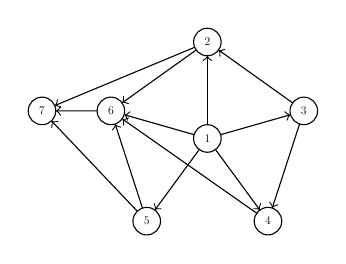
\begin{tikzpicture}[scale=0.35, transform shape, every node/.style={font=\large}]
       
        %add correct 4th here.
        
        % Define nodes with coordinates
\node[draw, circle, minimum size=1cm] (6) at (0, 0) {$1$};
\node[draw, circle, minimum size=1cm] (4) at (-6, 1) {$7$};
\node[draw, circle, minimum size=1cm] (2) at (2.2, -3) {$4$};
\node[draw, circle, minimum size=1cm] (7) at (-3.5, 1) {$6$};
\node[draw, circle, minimum size=1cm] (5) at (3.5, 1) {$3$};
\node[draw, circle, minimum size=1cm] (1) at (0, 3.5) {$2$};
\node[draw, circle, minimum size=1cm] (3) at (-2.2, -3) {$5$};

% Draw edges based on the given connections
\draw[->] (6) -- (1);
\draw[->] (6) -- (2);
\draw[->] (6) -- (3);
\draw[->] (6) -- (5);
\draw[->] (6) -- (7);


\draw[->] (2) -- (7);

\draw[->] (3) -- (4);

\draw[->] (3) -- (7);

\draw[<-] (4) -- (1);

\draw[<-] (4) -- (7);


\draw[->] (5) -- (1);
\draw[->] (5) -- (2);


\draw[<-] (7) -- (1);


        \end{tikzpicture}
      %  \caption{$H_{4}$}
       
   }

\vspace{1cm}

    \subfloat[$H_{5}$]{
        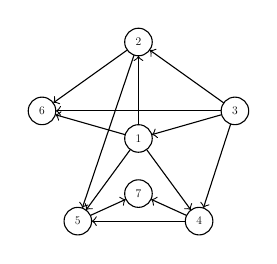
\begin{tikzpicture}[scale=0.35, transform shape, every node/.style={font=\large}]

        %add correct 5th here.
      % Define nodes with coordinates
\node[draw, circle, minimum size=1cm] (6) at (0, 0) {$1$};
\node[draw, circle, minimum size=1cm] (4) at (0, -2) {$7$};
\node[draw, circle, minimum size=1cm] (2) at (2.2, -3) {$4$};
\node[draw, circle, minimum size=1cm] (7) at (-3.5, 1) {$6$};
\node[draw, circle, minimum size=1cm] (5) at (3.5, 1) {$3$};
\node[draw, circle, minimum size=1cm] (1) at (0, 3.5) {$2$};
\node[draw, circle, minimum size=1cm] (3) at (-2.2, -3) {$5$};

% Draw edges based on the given connections
\draw[->] (6) -- (1);
\draw[->] (6) -- (2);
\draw[->] (6) -- (3);
\draw[->] (6) -- (7);
\draw[<-] (7) -- (5);

\draw[->] (1) -- (3);
\draw[->] (2) -- (3);

\draw[<-] (2) -- (5);






\draw[<-] (4) -- (2);
\draw[<-] (4) -- (3);


\draw[->] (5) -- (1);




\draw[<-] (6) -- (5);


\draw[<-] (7) -- (1);





        \end{tikzpicture}
      %  \caption{$H_{5}$}
        
    }
    \hfill
    \subfloat[$H_{6}$]{
        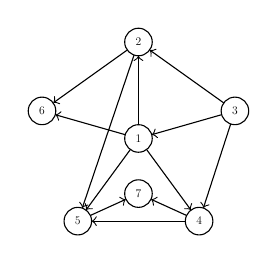
\begin{tikzpicture}[scale=0.35, transform shape, every node/.style={font=\large}]
       
        %add correct 6th here.
       % Define nodes with coordinates
\node[draw, circle, minimum size=1cm] (6) at (0, 0) {$1$};
\node[draw, circle, minimum size=1cm] (4) at (0, -2) {$7$};
\node[draw, circle, minimum size=1cm] (2) at (2.2, -3) {$4$};
\node[draw, circle, minimum size=1cm] (7) at (-3.5, 1) {$6$};
\node[draw, circle, minimum size=1cm] (5) at (3.5, 1) {$3$};
\node[draw, circle, minimum size=1cm] (1) at (0, 3.5) {$2$};
\node[draw, circle, minimum size=1cm] (3) at (-2.2, -3) {$5$};

% Draw edges based on the given connections
\draw[->] (6) -- (1);
\draw[->] (6) -- (2);
\draw[->] (6) -- (3);
\draw[->] (6) -- (7);


\draw[->] (1) -- (3);
\draw[->] (2) -- (3);



\draw[->] (3) -- (4);



\draw[<-] (4) -- (2);



\draw[->] (5) -- (1);
\draw[->] (5) -- (2);




\draw[<-] (6) -- (5);

\draw[<-] (7) -- (1);





        \end{tikzpicture}
     %   \caption{$H_{6}$}
      
    }
    \hfill
\subfloat[$H_{7}$]{
        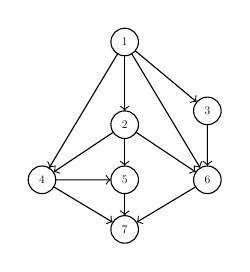
\begin{tikzpicture}[scale=0.35, transform shape, every node/.style={font=\large}]

        %add correct 7th here.
      % Define nodes with coordinates
 % Define nodes with coordinates
\node[draw, circle, minimum size=1cm] (2) at (0, -0.5) {$2$};
\node[draw, circle, minimum size=1cm] (1) at (0, 2.5) {$1$};
\node[draw, circle, minimum size=1cm] (3) at (3, 0) {$3$};
\node[draw, circle, minimum size=1cm] (4) at (-3, -2.5) {$4$};
\node[draw, circle, minimum size=1cm] (5) at (0, -2.5) {$5$};
\node[draw, circle, minimum size=1cm] (6) at (3, -2.5) {$6$};
\node[draw, circle, minimum size=1cm] (7) at (0, -4.3) {$7$};

% Draw edges based on the given connections
\draw[<-] (2) -- (1);
\draw[->] (1) -- (3);
\draw[<-] (6) -- (1);
\draw[<-] (4) -- (1);


\draw[->] (2) -- (4);
\draw[->] (2) -- (6);

\draw[->] (2) -- (5);
\draw[->] (3) -- (6);


\draw[<-] (5) -- (4);
\draw[->] (4) -- (7);


\draw[->] (5) -- (7);
\draw[->] (6) -- (7);

        \end{tikzpicture}
    %    \caption{$H_{7}$}
       
    }

\vspace{1cm}
     
   \subfloat[$H_{8}$]{
        \begin{tikzpicture}[scale=0.35, transform shape, every node/.style={font=\large}]
       
        %add correct 8th here.
       % Define nodes with coordinates
% Define nodes with coordinates
\node[draw, circle, minimum size=1cm] (2) at (0, -0.5) {$2$};
\node[draw, circle, minimum size=1cm] (1) at (0, 2.5) {$1$};
\node[draw, circle, minimum size=1cm] (3) at (3, 0) {$3$};
\node[draw, circle, minimum size=1cm] (4) at (-3, -2.5) {$4$};
\node[draw, circle, minimum size=1cm] (5) at (0, -2.5) {$5$};
\node[draw, circle, minimum size=1cm] (6) at (3, -2.5) {$6$};
\node[draw, circle, minimum size=1cm] (7) at (0, -4.3) {$7$};

% Draw edges based on the given connections
\draw[<-] (2) -- (1);
\draw[->] (1) -- (3);
\draw[<-] (6) -- (1);
\draw[<-] (4) -- (1);


\draw[->] (2) -- (4);
\draw[->] (2) -- (6);

\draw[->] (2) -- (5);
\draw[->] (3) -- (6);


\draw[<-] (5) -- (4);
\draw[->] (4) -- (7);



\draw[->] (6) -- (7);

\end{tikzpicture}
   %  \caption{$H_{8}$}
     
}
\hfill
\subfloat[$H_{9}$]{
        \begin{tikzpicture}[scale=0.35, transform shape, every node/.style={font=\large}]

        %add correct 9th here.
      % Define nodes with coordinates
 % Define nodes with coordinates
% Define nodes with coordinates
\node[draw, circle, minimum size=1cm] (2) at (0, -0.5) {$2$};
\node[draw, circle, minimum size=1cm] (1) at (0, 2.5) {$1$};
\node[draw, circle, minimum size=1cm] (3) at (3, 0) {$3$};
\node[draw, circle, minimum size=1cm] (4) at (-3, -2.5) {$4$};
\node[draw, circle, minimum size=1cm] (5) at (0, -2.5) {$5$};
\node[draw, circle, minimum size=1cm] (6) at (3, -2.5) {$6$};
\node[draw, circle, minimum size=1cm] (7) at (0, -4.3) {$7$};

% Draw edges based on the given connections
\draw[<-] (2) -- (1);
\draw[->] (1) -- (3);
\draw[<-] (6) -- (1);
\draw[<-] (4) -- (1);


\draw[->] (2) -- (4);
\draw[->] (2) -- (6);

\draw[->] (2) -- (5);
\draw[->] (3) -- (6);


\draw[<-] (5) -- (4);
\draw[->] (4) -- (7);





     \end{tikzpicture}
     %   \caption{$H_{9}$}
      
   }
\hfill
    \subfloat[$H_{10}$]{
        \begin{tikzpicture}[scale=0.35, transform shape, every node/.style={font=\large}]
       
        %add correct 10th here.
       % Define nodes with coordinates
% Define nodes with coordinates

% Define nodes with coordinates
\node[draw, circle, minimum size=1cm] (2) at (0, -0.5) {$2$};
\node[draw, circle, minimum size=1cm] (1) at (0, 2.5) {$1$};
\node[draw, circle, minimum size=1cm] (3) at (3, 0) {$3$};
\node[draw, circle, minimum size=1cm] (4) at (-3, -2.5) {$4$};
\node[draw, circle, minimum size=1cm] (5) at (0, -2.5) {$5$};
\node[draw, circle, minimum size=1cm] (6) at (3, -2.5) {$6$};
\node[draw, circle, minimum size=1cm] (7) at (0, -4.3) {$7$};

% Draw edges based on the given connections
\draw[<-] (2) -- (1);
\draw[->] (1) -- (3);
\draw[<-] (6) -- (1);
\draw[<-] (4) -- (1);


\draw[->] (2) -- (4);
\draw[->] (2) -- (6);

\draw[->] (2) -- (5);
\draw[->] (3) -- (6);


\draw[<-] (5) -- (4);
\draw[->] (4) -- (7);
\draw[->] (5) -- (7);

        \end{tikzpicture}
     %   \caption{$H_{10}$}
        
    } 
 \hfill
  \subfloat[$H_{11}$]{
 \begin{tikzpicture}[scale=0.35, transform shape, every node/.style={font=\large}]
\node[draw, text=black, circle, minimum size=1cm] (1) at (1.15, -2.5) {$1$};

\node[draw, circle, minimum size=1cm] (2) at (2.3, 0.6) {$2$};

\node[draw, circle, minimum size=1cm] (4) at (-3.7, 0.6) {$4$};

\node[draw, circle, minimum size=1cm] (3) at (-0.7, 3) {$3$};

\node[draw, circle, minimum size=1cm] (5) at (-2.95, -2.5) {$5$};

\node[draw, circle, minimum size=1cm] (6) at (-5.2, -4.7) {$6$};

\node[draw, circle, minimum size=1.2cm] (7) at (3.4, -4.7) {$7$};

\draw[->] (1) -- (2);
\draw[<-] (2) -- (3);
\draw[->] (3) -- (4);

\draw[->] (1) -- (5);
\draw[<-] (1) -- (3);
\draw[<-] (5) -- (4);

\draw[<-] (5) -- (2);
\draw[<-] (5) -- (3);
\draw[->] (1) -- (4);

\draw[->] (1) -- (6);
\draw[->] (4) -- (6);

\draw[->] (2) -- (7);
\draw[->] (5) -- (7);

 \end{tikzpicture}
%\caption{$H_{11}$}

  }
    \caption{Semi-transitive orientations of graphs in Figure \ref{fig:min-non-comp-part4} $($$H_{1}$ is not semi-transitive$)$} 
    \label{fig:min-non-comp-part4-semi-trans}
\end{figure}




Theorem \ref{minimal-nwrg-all-adj-thm} provides a characterization of the class of minimal non-word-representable graphs that contain an all-adjacent vertex.

\begin{theorem}
\label{minimal-nwrg-all-adj-thm}
Let \( G \) be a graph with \( n \) vertices, where a vertex \( x \in V(G) \) has degree \( (n-1) \), meaning \( x \) is adjacent to all other vertices in \( G \). Let \( H \) be the induced subgraph of \( G \) with \( V(H) = V(G) \setminus \{x\} \). Then, \( G \) is minimal non-word-representable if and only if both of the following conditions hold:
\begin{enumerate}
    \item \( H \) is minimal non-comparability.
    \item \( H \) is semi-transitive.
\end{enumerate}
\end{theorem}

\begin{proof}
Suppose \( H \) is a minimal non-comparability graph and is also semi-transitive. Since \( H \) is non-comparability, it follows from Lemma \ref{lemma_comp_wrg} that \( G \) is a non-word-representable graph. As \( H \) is minimal non-comparability, any proper induced subgraph \( H_1 \) of \( H \) is a comparability graph. Consider an induced subgraph \( G' \) of \( G \) where \( V(G') = V(H_1) \cup \{x\} \). Since \( H_1 \) is a comparability graph, Lemma \ref{lemma_comp_wrg} implies that \( G' \) is word-representable. Consequently, every proper induced subgraph of \( G \) containing the vertex \( x \) is word-representable. Furthermore, since \( H \) is semi-transitive, it follows from Theorem \ref{wrg=semi} that \( H \) is word-representable. As word-representable graphs are hereditary, every proper induced subgraph of \( G \) is word-representable, confirming that \( G \) is a minimal non-word-representable graph.


\begin{lemma}
\label{lemma_comp_wrg}
\cite{onrepgraphs}  
Let \( G \) be a graph with \( n \) vertices, where a vertex \( x \in V(G) \) has degree \( (n-1) \). Let \( H \) be the induced subgraph of \( G \) with \( V(H) = V(G) \setminus \{x\} \). Then, \( G \) is word-representable if and only if \( H \) is a comparability graph.
\end{lemma}

Suppose \( G \) is a minimal non-word-representable graph with an all-adjacent vertex \( x \in V(G) \). Since \( G \) is minimal, every proper induced subgraph of \( G \) is word-representable. By Theorem \ref{wrg=semi}, it follows that \( H \) is semi-transitive. Now, assume \( H \) is a comparability graph. By Lemma \ref{lemma_comp_wrg}, \( G \) must then be word-representable, contradicting the assumption that \( G \) is non-word-representable. Hence, \( H \) is a non-comparability graph. Next, consider the case where \( H \) fails to be a minimal non-comparability graph.
 Then, there exists a proper induced subgraph \( H_2 \) of \( H \) that is also non-comparability. The induced subgraph of \( G \) formed by the vertex set \( V(H_2) \cup \{x\} \subset V(G) \) would then be non-word-representable by Lemma \ref{lemma_comp_wrg}, contradicting the minimality of \( G \). Thus, \( H \) must be a minimal non-comparability graph.
\end{proof}



We have identified all the minimal non-comparability graphs that are semi-transitive. Therefore, by applying Theorem \ref{minimal-nwrg-all-adj-thm}, if we add an all-adjacent vertex to each of these minimal non-comparability graphs that are semi-transitive, we obtain all the minimal non-word-representable graphs that contain an all-adjacent vertex. 
\paragraph{}
In the following section, we identify the minimal non-comparability graphs that are not semi-transitive. They are the graphs which falls in the intersection of minimal non-comparability graphs and minimal non-word-representable graphs.


\section{Minimal non-comparability graphs that are not semi-transitive}
\label{section-minimal-non-semi-trans}

In this section, we determine which graphs in the list of minimal non-comparability graphs are not semi-transitive.

\begin{theorem}
\label{theorem-g9n}
    The graph class \( G_{n}^{9} \), depicted in Figure \ref{g9n}, forms an infinite subclass of minimal non-word-representable graphs.
\end{theorem}

\begin{proof}

    Let $G \in G_{n}^{9}$ be an arbitrary graph. If $G$ is word-representable, then by Theorem \ref{wrg=semi} and Theorem \ref{source_vertex}, there exists a semi-transitive orientation of $G'$ where vertex $d$ is the source (i.e., all edges incident to $d$ are oriented away from it). Consider such an orientation where $d$ is the source. By symmetry between vertices $a$ and $b$, we may assume without loss of generality that the edge between them is oriented as $a \rightarrow b$.


\begin{note}
    The orientations $a \rightarrow c$ and $c \rightarrow b$ are not possible, as the path $d \rightarrow a \rightarrow c \rightarrow b$ violates semi-transitivity. 
\end{note}

\begin{note}
    Similarly, $b \rightarrow c$ and $c \rightarrow a$ are not possible, as the path $d \rightarrow b \rightarrow c \rightarrow a$ violates semi-transitivity. 
\end{note}

Thus, the only remaining valid orientations are $a \rightarrow c$, $b \rightarrow c$ and $c \rightarrow a$, $c \rightarrow b$.

\subsubsection*{\textnormal{\textbf{Case $1$:} $a \rightarrow c$, $b \rightarrow c$}}
%\noindent \textbf{\underline{Case 1:}} $a \rightarrow c$, $b \rightarrow c$.  \\
\medskip
The edge between $1$ and $b$ must be oriented as $1 \rightarrow b$. If $b \rightarrow 1$, then the path $d \rightarrow a \rightarrow b \rightarrow 1$ violates semi-transitivity.
\begin{observation}
    In a semi-transitive orientation of $G$, where $d$ is the source and the edges among $a, c$, and $b$ are oriented as $a \rightarrow c$, $b \rightarrow c$, and $a \rightarrow b$, the edges from any vertex $i$, $2 \leq i \leq (n-1)$, to $a$ and $b$ must be oriented as $i \rightarrow a$ and $i \rightarrow b$.
\end{observation}

\begin{proof}
    The following cases can be ruled out:
    \begin{enumerate}
        \item $a \rightarrow i$ and $i \rightarrow b$, since the path $a \rightarrow i \rightarrow b \rightarrow c$ violates semi-transitivity.
        \item $b \rightarrow i$ and $i \rightarrow a$, since the path $b \rightarrow i \rightarrow a \rightarrow c$ violates semi-transitivity.
    \end{enumerate}
    Thus, the remaining possibilities are:
    \begin{enumerate}
        \item $a \rightarrow i$ and $b \rightarrow i$.
        \item $i \rightarrow a$ and $i \rightarrow b$.
    \end{enumerate}
    
    For $i = 2$, $b \rightarrow 2$ is not valid, as the path $d \rightarrow 1 \rightarrow b \rightarrow 2$ violates semi-transitivity. Hence, the valid orientation for $i = 2$ is $i \rightarrow a$ and $i \rightarrow b$. Now, assume that at least one vertex $i$ has the orientation $a \rightarrow i$ and $b \rightarrow i$. Let $i$ be the smallest such vertex. Then, the path $d \rightarrow (i-1) \rightarrow b \rightarrow i$ violates semi-transitivity, leading to a contradiction. Thus, the only valid orientation is $i \rightarrow a$ and $i \rightarrow b$.
\end{proof}

\begin{note}
\label{a-n}
    The edge between $a$ and $n$ cannot be oriented as $a \rightarrow n$ since the path $d \rightarrow (n-1) \rightarrow a \rightarrow n$ violates semi-transitivity.
\end{note}

\begin{note}
\label{n-a}
    The edge between $a$ and $n$ cannot be oriented as $n \rightarrow a$ since the path $d \rightarrow n \rightarrow a \rightarrow b$ violates semi-transitivity.
\end{note}

From Notes \ref{a-n} and \ref{n-a}, we reach a contradiction. Hence, no semi-transitive orientation exists for $G$. Since $G$ is a minimal non-comparability graph, every proper induced subgraph of $G$ is word-representable, proving its minimality.

\subsubsection*{\textnormal{\textbf{Case $2$:} $c \rightarrow a$, $c \rightarrow b$}}
\medskip
The edge between $1$ and $b$ must be oriented as $1 \rightarrow b$. If $b \rightarrow 1$, the path $d \rightarrow a \rightarrow b \rightarrow 1$ violates semi-transitivity.

\begin{note}
    In a semi-transitive orientation of $G$, where $d$ is the source and the edges among $a, c$, and $b$ are oriented as $c \rightarrow a$, $c \rightarrow b$, and $a \rightarrow b$, the edges from any vertex $i$, $2 \leq i \leq (n-1)$, to $a$ and $b$ must be oriented as $i \rightarrow a$ and $i \rightarrow b$.
\end{note}

\begin{proof}
    The following cases can be ruled out:
    \begin{enumerate}
        \item $a \rightarrow i$ and $i \rightarrow b$, since the path $c \rightarrow a \rightarrow i \rightarrow b$ violates semi-transitivity.
        \item $b \rightarrow i$ and $i \rightarrow a$, since the path $c \rightarrow b \rightarrow i \rightarrow a$ violates semi-transitivity.
    \end{enumerate}
    Thus, the remaining possibilities are:
    \begin{enumerate}
        \item $a \rightarrow i$ and $b \rightarrow i$.
        \item $i \rightarrow a$ and $i \rightarrow b$.
    \end{enumerate}
    
    For $i = 2$, $b \rightarrow 2$ is not valid, as the path $d \rightarrow 1 \rightarrow b \rightarrow 2$ violates semi-transitivity. Hence, the valid orientation for $i = 2$ is $i \rightarrow a$ and $i \rightarrow b$. Suppose at least one vertex $i$ has the orientation $a \rightarrow i$ and $b \rightarrow i$. Let $i$ be the smallest such vertex. Then, the path $d \rightarrow (i-1) \rightarrow b \rightarrow i$ violates semi-transitivity, leading to a contradiction. Thus, the only valid orientation is $i \rightarrow a$ and $i \rightarrow b$.
\end{proof}

\begin{note}
\label{a-ncase2}
    The edge between $a$ and $n$ cannot be oriented as $a \rightarrow n$ since the path $d \rightarrow (n-1) \rightarrow a \rightarrow n$ violates semi-transitivity.
\end{note}

\begin{note}
\label{n-acase2}
    The edge between $a$ and $n$ cannot be oriented as $n \rightarrow a$ since the path $d \rightarrow n \rightarrow a \rightarrow b$ violates semi-transitivity.
\end{note}

From Notes \ref{a-ncase2} and \ref{n-acase2}, we reach a contradiction. Hence, no semi-transitive orientation exists for $G$. Since $G$ is a minimal non-comparability graph, every proper induced subgraph of $G$ is word-representable, proving its minimality.

\end{proof}

\begin{theorem}
\label{theorem-g4n}
    The graph class \( G_{n}^{4} \), depicted in Figure \ref{g4n}, forms an infinite subclass of minimal non-word-representable graphs.
\end{theorem}

\begin{proof}
 Consider an arbitrary graph \( G \in G_{n}^{4} \). Assume \( G \) is word-representable. By Theorem \ref{wrg=semi} and Theorem \ref{source_vertex}, it follows that there exists a semi-transitive orientation of \( G \) in which vertex 1 serves as the source, meaning that all edges incident to vertex 1 are oriented away from it. Let \( G' \) denote such a directed version of the graph \( G \), where \( G' \) is semi-transitive and every edge incident to vertex $1$ is directed away from it. Consider the induced subgraph \( G'' \), where \( V(G'') = V(G') \setminus \{x,y\} \). If \( G'' \) is not semi-transitive, then it must follow that \( G' \) is also not semi-transitive, as the same violation of semi-transitivity would appear in \( G' \). Therefore, \( G'' \) must be semi-transitive. Next, we examine the undirected version of \( G'' \), denoted as \( G''_U \). Lemma \ref{semi-trans_of_G''_U} addresses the number of possible semi-transitive orientations of \( G''_U \) with vertex $1$ as the source vertex.
\begin{figure}[htbp]
    \centering
\subfloat[Case: $2 \rightarrow3$, $(2n+1) \rightarrow 2n$.]{

  \begin{tikzpicture}[scale=0.6, transform shape, every node/.style={font=\large}]

\node[draw, circle, minimum size=1.4cm] (1) at (1.15, -2.5) {$1$};
\node[draw, circle, minimum size=1.4cm] (2) at (3.4, 0) {$2$};
\node[draw, circle, minimum size=1.4cm] (2n) at (-3.9, 0) {$2n$};
\node[draw, circle, minimum size=1.4cm] (3) at (3.37, 2.3) {$3$};
\node[draw, circle, minimum size=1.4cm] (r1) at (-3.9, 2.3) {$2n-1$};
\node[draw, circle, minimum size=1.4cm] (4) at (1.2, 4) {$4$};
\node[draw, circle, minimum size=1.4cm] (r) at (-1.7, 4) {};
\node[draw, circle, minimum size=1.4cm] (2n+1) at (-1.65, -2.5) {$2n+1$};

\draw[->] (1) -- (2);
\draw[->] (2) -- (3);
\draw[<-] (3) -- (4);
\draw[->] (4) -- (r) node[midway, above, yshift=5pt] {. . . . . . .};
\draw[->] (1) -- (3);
\draw[->] (1) -- (4);
\draw[->] (1) -- (4);
\draw[->] (1) -- (r);
\draw[->] (1) -- (r);
\draw[->] (1) -- (r1);
\draw[->] (1) -- (2n);
\draw[->] (1) -- (r);
\draw[->] (1) -- (2n+1);
\draw[->] (2n+1) -- (2);
\draw[->] (2n+1) -- (3);
\draw[->] (2n+1) -- (4);
\draw[->] (2n+1) -- (r);
\draw[->] (2n+1) -- (r1);
\draw[->] (2n+1) -- (2n);
\draw[->] (2n+1) -- (2);
\draw[->] (r) -- (r1);
\draw[->] (2n) -- (r1);



\end{tikzpicture}
% \subcaption{Case: $2 \rightarrow3$, $(2n+1) \rightarrow 2n$.}
 \label{G''UA}
 }
\hfill
\subfloat[Case: $2 \rightarrow3$, $2n \rightarrow (2n+1)$.]{

  \begin{tikzpicture}[scale=0.6, transform shape, every node/.style={font=\large}]

\node[draw, circle, minimum size=1.4cm] (1) at (1.15, -2.5) {$1$};
\node[draw, circle, minimum size=1.4cm] (2) at (3.4, 0) {$2$};
\node[draw, circle, minimum size=1.4cm] (2n) at (-3.9, 0) {$2n$};
\node[draw, circle, minimum size=1.4cm] (3) at (3.37, 2.3) {$3$};
\node[draw, circle, minimum size=1.4cm] (r1) at (-3.9, 2.3) {$2n-1$};
\node[draw, circle, minimum size=1.4cm] (4) at (1.2, 4) {$4$};
\node[draw, circle, minimum size=1.4cm] (r) at (-1.7, 4) {};
\node[draw, circle, minimum size=1.4cm] (2n+1) at (-1.65, -2.5) {$2n+1$};

\draw[->] (1) -- (2);
\draw[->] (2) -- (3);
\draw[<-] (3) -- (4);
\draw[->] (4) -- (r) node[midway, above, yshift=5pt] {. . . . . . .};
\draw[->] (1) -- (3);
\draw[->] (1) -- (4);
\draw[->] (1) -- (4);
\draw[->] (1) -- (r);
\draw[->] (1) -- (r);
\draw[->] (1) -- (r1);
\draw[->] (1) -- (2n);
\draw[->] (1) -- (r);
\draw[->] (1) -- (2n+1);
\draw[<-] (2n+1) -- (2);
\draw[<-] (2n+1) -- (3);
\draw[<-] (2n+1) -- (4);
\draw[<-] (2n+1) -- (r);
\draw[<-] (2n+1) -- (r1);
\draw[<-] (2n+1) -- (2n);
\draw[<-] (2n+1) -- (2);
\draw[->] (r) -- (r1);
\draw[->] (2n) -- (r1);



\end{tikzpicture}
 %\subcaption{Case: $2 \rightarrow3$, $2n \rightarrow (2n+1)$.}
 \label{G''UB}
}
    
    \vspace{1cm} % Space between the two rows

\subfloat[Case: $3 \rightarrow 2$, $(2n+1) \rightarrow 2n$.]{

  \begin{tikzpicture}[scale=0.6, transform shape, every node/.style={font=\large}]

\node[draw, circle, minimum size=1.4cm] (1) at (1.15, -2.5) {$1$};
\node[draw, circle, minimum size=1.4cm] (2) at (3.4, 0) {$2$};
\node[draw, circle, minimum size=1.4cm] (2n) at (-3.9, 0) {$2n$};
\node[draw, circle, minimum size=1.4cm] (3) at (3.37, 2.3) {$3$};
\node[draw, circle, minimum size=1.4cm] (r1) at (-3.9, 2.3) {$2n-1$};
\node[draw, circle, minimum size=1.4cm] (4) at (1.2, 4) {$4$};
\node[draw, circle, minimum size=1.4cm] (r) at (-1.7, 4) {};
\node[draw, circle, minimum size=1.4cm] (2n+1) at (-1.65, -2.5) {$2n+1$};

\draw[->] (1) -- (2);
\draw[->] (3) -- (2);
\draw[->] (3) -- (4);
\draw[<-] (4) -- (r) node[midway, above, yshift=5pt] {. . . . . . .};
\draw[->] (1) -- (3);
\draw[->] (1) -- (4);
\draw[->] (1) -- (4);
\draw[->] (1) -- (r);
\draw[->] (1) -- (r);
\draw[->] (1) -- (r1);
\draw[->] (1) -- (2n);
\draw[->] (1) -- (r);
\draw[->] (1) -- (2n+1);
\draw[->] (2n+1) -- (2);
\draw[->] (2n+1) -- (3);
\draw[->] (2n+1) -- (4);
\draw[->] (2n+1) -- (r);
\draw[->] (2n+1) -- (r1);
\draw[->] (2n+1) -- (2n);
\draw[->] (2n+1) -- (2);
\draw[<-] (r) -- (r1);
\draw[<-] (2n) -- (r1);



\end{tikzpicture}
% \subcaption{Case: $3 \rightarrow 2$, $(2n+1) \rightarrow 2n$.}
 \label{G''UC}
 }
 \hfill
\subfloat[Case: $3 \rightarrow2$, $2n \rightarrow (2n+1)$.]{

  \begin{tikzpicture}[scale=0.6, transform shape, every node/.style={font=\large}]

\node[draw, circle, minimum size=1.4cm] (1) at (1.15, -2.5) {$1$};
\node[draw, circle, minimum size=1.4cm] (2) at (3.4, 0) {$2$};
\node[draw, circle, minimum size=1.4cm] (2n) at (-3.9, 0) {$2n$};
\node[draw, circle, minimum size=1.4cm] (3) at (3.37, 2.3) {$3$};
\node[draw, circle, minimum size=1.4cm] (r1) at (-3.9, 2.3) {$2n-1$};
\node[draw, circle, minimum size=1.4cm] (4) at (1.2, 4) {$4$};
\node[draw, circle, minimum size=1.4cm] (r) at (-1.7, 4) {};
\node[draw, circle, minimum size=1.4cm] (2n+1) at (-1.65, -2.5) {$2n+1$};

\draw[->] (1) -- (2);
\draw[->] (3) -- (2);
\draw[->] (3) -- (4);
\draw[<-] (4) -- (r) node[midway, above, yshift=5pt] {. . . . . . .};
\draw[->] (1) -- (3);
\draw[->] (1) -- (4);
\draw[->] (1) -- (4);
\draw[->] (1) -- (r);
\draw[->] (1) -- (r);
\draw[->] (1) -- (r1);
\draw[->] (1) -- (2n);
\draw[->] (1) -- (r);
\draw[->] (1) -- (2n+1);
\draw[<-] (2n+1) -- (2);
\draw[<-] (2n+1) -- (3);
\draw[<-] (2n+1) -- (4);
\draw[<-] (2n+1) -- (r);
\draw[<-] (2n+1) -- (r1);
\draw[<-] (2n+1) -- (2n);
\draw[<-] (2n+1) -- (2);
\draw[<-] (r) -- (r1);
\draw[<-] (2n) -- (r1);



\end{tikzpicture}
%\subcaption{Case: $3 \rightarrow2$, $2n \rightarrow (2n+1)$.}
 \label{G''UD}
}
    \caption{Four semi-transitive orientations of $G''_{U}$, with $1$ as a source.}
    \label{fig:4orientationsofG''U}
\end{figure}

 \begin{observation}
     \label{semi-trans_of_G''_U}
    There are exactly four semi-transitive orientations of the graph \( G''_U \), with vertex $1$ as a source, as illustrated in Figure \ref{fig:4orientationsofG''U}.
 \end{observation}

Lemma \ref{case1_if_2n+1to2n} and Lemma \ref{case2_if_2n+1to2n} gives the proof for Observation \ref{semi-trans_of_G''_U}. The orientation of the edge \( \{2,3\} \in E(G''_{U}) \) can either be \( 2 \rightarrow 3 \) or \( 3 \rightarrow 2 \). We will examine the possible semi-transitive orientations of \( G''_{U} \) for both cases.
    
    \vspace{0.5em}
    \subsubsection*{\textnormal{\textbf{Case 1:} \( 2 \rightarrow 3 \)}}
    \medskip
    \begin{lemma}
    \label{case1lemma_i_i+1}
        If \( G''_{U} \) is oriented with vertex 1 as the source and has the orientation \( 2 \rightarrow 3 \), then to achieve a semi-transitive orientation for \( G''_{U} \), any even-numbered vertex \( i \), where \( 4 \leq i \leq 2n-2 \), must have the following orientation:
        \begin{enumerate}
            \item \( i \rightarrow (i+1) \)
            \item \( i \rightarrow (i-1) \)
        \end{enumerate}
    \end{lemma}
    
    \begin{proof}
        Consider the case when \( i = 4 \). If the orientation is \( 3 \rightarrow 4 \), the path \( 1 \rightarrow 2 \rightarrow 3 \rightarrow 4 \) violates semi-transitivity. Thus, the valid orientation is \( 4 \rightarrow 3 \). Similarly, if the orientation is \( 5 \rightarrow 4 \), the path \( 1 \rightarrow 5 \rightarrow 4 \rightarrow 3 \) violates semi-transitivity, so the correct orientation is \( 4 \rightarrow 5 \). Therefore, Lemma \ref{case1lemma_i_i+1} holds when \( i = 4 \). Now, assume that Lemma \ref{case1lemma_i_i+1} holds for \( i = j \), where \( j \) is even, \( j > 4 \), and \( j \leq 2k-4 \), i.e., the orientations \( j \rightarrow (j-1) \) and \( j \rightarrow (j+1) \) are valid. Consider the case when \( i = j+2 \). If the orientation is \( (j+1) \rightarrow (j+2) \), then the path \( 1 \rightarrow j \rightarrow (j+1) \rightarrow (j+2) \) violates semi-transitivity. Thus, the valid orientation is \( (j+2) \rightarrow (j+1) \). On the other hand, if the orientation is \( (j+3) \rightarrow (j+2) \), the path \( 1 \rightarrow (j+3) \rightarrow (j+2) \rightarrow (j+1) \) violates semi-transitivity, so the correct orientation is \( (j+2) \rightarrow (j+3) \).
    \end{proof}
    
    \begin{note}
        If \( (2n-1) \rightarrow 2n \), then the path \( 1 \rightarrow (2n-2) \rightarrow (2n-1) \rightarrow 2n \) violates semi-transitivity. Thus, the valid orientation is \( 2n \rightarrow (2n-1) \).
    \end{note}

    \begin{lemma}
        \label{case1_if_2n+1to2n}
        There are only two semi-transitive orientations possible under the case of orienting the edge $\{2,3\} \in E(G''_{U})$ as $2 \rightarrow 3$, based on the following two conditions. For \( i \), \( 2 \leq i \leq 2n-1 \),
        \begin{enumerate}
            \item If \( (2n+1) \rightarrow 2n \), then \( (2n+1) \rightarrow i \).
            \item If \( 2n \rightarrow (2n+1) \), then \( i \rightarrow (2n+1) \).
        \end{enumerate}
        They are shown in Figure \ref{G''UA} and Figure \ref{G''UB}.
    \end{lemma}

    \begin{proof}
       Suppose we orient \( (2n+1) \to 2n \). Consider the case when \( i = 2 \). If \( 2 \to (2n+1) \), then the path \( 1 \to 2 \to (2n+1) \to 2n \) violates semi-transitivity. Therefore, the valid orientation is \( (2n+1) \to 2 \). Now, assume for \( i = j \), the orientation is \( (2n+1) \to j \). When \( i = j+1 \), if the orientation is \( (j+1) \to (2n+1) \), then the path \( 1 \to (j+1) \to (2n+1) \to 2 \) violates semi-transitivity. Hence, the valid orientation is \( (2n+1) \to (j+1) \). Now, consider the orientation \( 2n \to (2n+1) \). Examining the case when \( i = 2 \), if the edge is directed as \( (2n+1) \to 2 \), then the path \( 1 \to 2n \to (2n+1) \to 2 \) violates the semi-transitivity condition. Consequently, the correct orientation must be \( 2 \to (2n+1) \). Suppose for \( i = j \), the orientation is \( j \to (2n+1) \). When \( i = j+1 \), if the orientation is \( (2n+1) \to (j+1) \), the path \( 1 \to 2 \to (2n+1) \to (j+1) \) violates semi-transitivity. Hence, the correct orientation is \( (2n+1) \to (j+1) \).
    \end{proof}

    \vspace{1em}
    \subsubsection*{\textnormal{\textbf{Case 2:} \( 3 \rightarrow 2 \)}}
    \medskip
    \begin{lemma}
    \label{case2lemma_i_i+1}
        If \( G''_{U} \) is oriented with vertex 1 as the source and has the orientation \( 3 \rightarrow 2 \), then to achieve a semi-transitive orientation for \( G''_{U} \), any even-numbered vertex \( i \), where \( 4 \leq i \leq 2n-2 \), must have the following orientation:
        \begin{enumerate}
            \item \( i \leftarrow (i+1) \)
            \item \( i \leftarrow (i-1) \)
        \end{enumerate}
    \end{lemma}

    \begin{proof}
        Consider the case when \( i = 4 \). If the orientation is \( 4 \rightarrow 3 \), the path \( 1 \rightarrow 4 \rightarrow 3 \rightarrow 2 \) violates semi-transitivity. Hence, the valid orientation is \( 3 \rightarrow 4 \). Similarly, if the orientation is \( 4 \rightarrow 5 \), the path \( 1 \rightarrow 3 \rightarrow 4 \rightarrow 5 \) violates semi-transitivity, so the correct orientation is \( 5 \rightarrow 4 \). Thus, Lemma \ref{case2lemma_i_i+1} holds when \( i = 4 \). Now, assume that Lemma \ref{case2lemma_i_i+1} holds for \( i = j \), where \( j \) is even, \( j > 4 \), and \( j \leq 2n-4 \), i.e., the orientations \( j \leftarrow (j-1) \) and \( j \leftarrow (j+1) \) are valid. Consider the case when \( i = j+2 \). If the orientation is \( (j+1) \leftarrow (j+2) \), the path \( 1 \rightarrow (j+2) \rightarrow (j+1) \rightarrow j \) violates semi-transitivity. Therefore, the valid orientation is \( (j+2) \leftarrow (j+1) \). If the orientation is \( (j+3) \leftarrow (j+2) \), the path \( 1 \rightarrow (j+1) \rightarrow (j+2) \rightarrow (j+3) \) violates semi-transitivity, so the correct orientation is \( (j+2) \leftarrow (j+3) \).
    \end{proof}

    \begin{note}
        If \( (2n-1) \leftarrow 2n \), the path \( 1 \rightarrow 2n \rightarrow (2n-1) \rightarrow (2n-2) \) violates semi-transitivity. Thus, the valid orientation is \( 2n \leftarrow (2n-1) \).
    \end{note}
    
    \begin{lemma}
        \label{case2_if_2n+1to2n}
        There are only two semi-transitive orientations possible under the case of orienting the edge $\{2,3\} \in E(G''_{U})$ as $3 \rightarrow 2$, based on the following two conditions. For \( i \), \( 2 \leq i \leq 2n-1 \),
        \begin{enumerate}
            \item If \( (2n+1) \rightarrow 2n \), then \( (2n+1) \rightarrow i \).
            \item If \( 2n \rightarrow (2n+1) \), then \( i \rightarrow (2n+1) \).
        \end{enumerate}
        They are shown in Figure \ref{G''UC} and Figure \ref{G''UD}.
    \end{lemma}

    \begin{proof}
        Suppose we orient \( (2n+1) \rightarrow 2n \) in \( G''_{P} \). Consider the case when \( i = 2 \). If \( 2 \rightarrow (2n+1) \), the path \( 1 \rightarrow 2 \rightarrow (2n+1) \rightarrow 2n \) violates semi-transitivity. Thus, the valid orientation is \( (2n+1) \rightarrow 2 \). Suppose for \( i = j \), the orientation is \( (2n+1) \rightarrow j \). When \( i = j+1 \), if the orientation is \( (j+1) \rightarrow (2n+1) \), then the path \( 1 \rightarrow (j+1) \rightarrow (2n+1) \rightarrow 2 \) violates semi-transitivity, and hence the valid orientation is \( (2n+1) \rightarrow (j+1) \). Suppose we orient \( 2n \rightarrow (2n+1) \) . Consider the case when \( i = 2 \). If \( (2n+1) \rightarrow 2 \), the path \( 1 \rightarrow 2n \rightarrow (2n+1) \rightarrow 2 \) violates semi-transitivity. Thus, the valid orientation is \( 2 \rightarrow (2n+1) \). Suppose for \( i = j \), the orientation is \( j \rightarrow (2n+1) \). When \( i = j+1 \), if the orientation is \( (2n+1) \rightarrow (j+1) \), the path \( 1 \rightarrow 2 \rightarrow (2n+1) \rightarrow (j+1) \) violates semi-transitivity. Hence, the correct orientation is \( (2n+1) \rightarrow (j+1) \).
    \end{proof}


   The graph \( G' \) is an extension of the four types of graphs depicted in Figure \ref{fig:4orientationsofG''U}. To construct \( G' \), two additional vertices, \( x \) and \( y \), are introduced, along with the edges \( \{1, x\} \), \( \{2n, x\} \), \( \{2, y\} \), and \( \{2n+1, y\} \). The orientation of the edge \( \{1, x\} \) is predetermined as \( 1 \to x \). We demonstrate that none of these extensions preserve the semi-transitivity of \( G' \), thereby leading to a contradiction.

      
    \begin{enumerate}
        \item Extending the graph in Figure \ref{G''UA}. 
        \par
      The edge $\{2n, x\}$, cannot be oriented as $2n \rightarrow x$, as the path $1 \rightarrow (2n+1) \rightarrow 2n \rightarrow x$ violates semi-transitivity. The edge $\{2n, x\}$, cannot be oriented as $x \rightarrow 2n$, as the path $1 \rightarrow x \rightarrow 2n \rightarrow (2n-1)$ violates semi-transitivity. Hence, we do not get a semi-transitive $G'$.  The orientation of the edge $\{1, x\}$ is known, which is $1 \rightarrow x$.  
\vspace{0.2cm}
        \item Extending the graph in Figure \ref{G''UB}. 
        \par
        The orientations of the edges \( \{2, y\} \) and \( \{2n+1, y\} \) can be of four types, and none of them maintains semi-transitivity.
        \begin{enumerate}
            \item If the orientations were $2 \rightarrow y$, and $y \rightarrow (2n+1)$, the path $1 \rightarrow 2 \rightarrow y \rightarrow (2n+1)$ violates semi-transitivity.
             \item If the orientations were $2 \rightarrow y$, and $(2n+1) \rightarrow y$, the path $2 \rightarrow 3 \rightarrow (2n+1) \rightarrow y$ violates semi-transitivity.
              \item If the orientations were $y\rightarrow 2$, and $y \rightarrow (2n+1)$, the path $y \rightarrow 2 \rightarrow 3 \rightarrow (2n+1)$ violates semi-transitivity.
               \item If the orientations were $y \rightarrow 2$, and $(2n+1) \rightarrow y$, the path $1 \rightarrow (2n+1) \rightarrow y \rightarrow 2$ violates semi-transitivity.
        \end{enumerate}
\vspace{0.2cm}
        \item Extending the graph in Figure \ref{G''UC}. 
        \par
        \par
        The orientations of the edges \( \{2, y\} \) and \( \{2n+1, y\} \) can be of four types, and none of them maintains semi-transitivity.
        \begin{enumerate}
            \item If the orientations were $2 \rightarrow y$, and $y \rightarrow (2n+1)$, the path $1 \rightarrow 2 \rightarrow y \rightarrow (2n+1)$ violates semi-transitivity.
             \item If the orientations were $2 \rightarrow y$, and $(2n+1) \rightarrow y$, the path $(2n+1) \rightarrow 3 \rightarrow 2 \rightarrow y$ violates semi-transitivity.
              \item If the orientations were $y\rightarrow 2$, and $y \rightarrow (2n+1)$, the path $y \rightarrow (2n+1) \rightarrow 3 \rightarrow 2$ violates semi-transitivity.
               \item If the orientations were $y \rightarrow 2$, and $(2n+1) \rightarrow y$, the path $1 \rightarrow (2n+1) \rightarrow y \rightarrow 2$ violates semi-transitivity.
        \end{enumerate}
        \vspace{0.2cm}
        \item Extending the graph in Figure \ref{G''UD}. 
        \par
        The edge $\{2n, x\}$, cannot be oriented as $2n \rightarrow x$, as the path $1 \rightarrow (2n-1) \rightarrow 2n \rightarrow x$ violates semi-transitivity. The edge $\{2n, x\}$, cannot be oriented as $x \rightarrow 2n$, as the path $1 \rightarrow x \rightarrow 2n \rightarrow (2n+1)$ violates semi-transitivity. Hence, we do not get a semi-transitive $G'$.
    \end{enumerate}
\end{proof}

\begin{remark}
    The graph $H_{1}$, depicted in Figure \ref{$H_{1}$}, is a minimal non-word-representable graph. The proof of this result has already been provided in \cite{kitaev2023humanverifiable}, and therefore, we do not include it here.
\end{remark}




\section{Concluding remarks}
\label{section-conclusion}

We have determined the set of all graphs that lie in the intersection of minimal non-comparability graphs and minimal non-word-representable graphs. We identify that this intersection consists of two infinite families of graphs, namely \( G_n^9 \) and \( G_n^4 \), as well as the graph \( H_1 \), which are illustrated in Figure \ref{g9n}, Figure \ref{g4n}, and Figure \ref{$H_{1}$}, respectively. Furthermore, we classify all minimal non-comparability graphs into two categories: those that are semi-transitive and those that are not. Building on this classification, we identify and characterize the set of all minimal non-word-representable graphs containing an all-adjacent vertex. As a byproduct of our study, we discover several minimal non-word-representable graphs.


\bibliography{references}


\end{document}




\begin{thebibliography}{99}

\bibitem{Ahn2022} 
Ahn, J., Jaffke, L., Kwon, O., Lima, P.T.: Well-partitioned chordal graphs. 
Discrete Math. \textbf{345}(10), 112985 (2022). 
\doi{10.1016/j.disc.2022.112985}

\bibitem{Blair1993} 
Blair, J.R.S., Peyton, B.: An Introduction to Chordal Graphs and Clique Trees. 
In: George, A., Gilbert, J.R., Liu, J.W.H. (eds.) Graph Theory and Sparse Matrix Computation, pp. 1--29. 
Springer, New York (1993).

\bibitem{Bender1985} 
Bender, E., Richmond, L., Wormald, N.: Almost all chordal graphs split. 
J. Aust. Math. Soc. \textbf{38}, 214--221 (1985). 
\doi{10.1017/S1446788700023077}

\bibitem{Collins2014} 
Collins, A., Kitaev, S., Lozin, V.: New results on word-representable graphs. 
Discrete Appl. Math. \textbf{216}, 201--209 (2014). 
\doi{10.1016/j.dam.2014.10.024}

\bibitem{Cornuejols2000} 
Cornuéjols, G., Liu, Y., Vušković, K.: Recognition of even-hole-free graphs. 
Discrete Math. \textbf{224}(1--3), 55--61 (2000).

\bibitem{Farber1987} 
Farber, M., Jamison, R.E.: Applications of perfect graphs to communication complexity. 
J. Comb. Theory Ser. B \textbf{43}(1), 50--63 (1987).

\bibitem{Gallai1967} 
Gallai, T.: Transitiv orientierbare Graphen. 
Acta Math. Acad. Sci. Hung. \textbf{18}, 25--66 (1967).

\bibitem{Golumbic2004} 
Golumbic, M.C.: Chapter 4 - Triangulated graphs. 
In: Algorithmic Graph Theory and Perfect Graphs, Ann. Discrete Math., vol. 57, pp. 81--104. 
Elsevier (2004). 
\doi{10.1016/S0167-5060(04)80052-9}

\bibitem{Grotschel1981} 
Grötschel, M., Lovász, L., Schrijver, A.: The ellipsoid method and its consequences in combinatorial optimization. 
Combinatorica \textbf{1}(2), 169--197 (1981).

\bibitem{Hougardy2006} 
Hougardy, S.: Classes of perfect graphs. 
Discrete Math. \textbf{306}(19), 2529--2571 (2006). 
\doi{10.1016/j.disc.2006.05.021}

\bibitem{Kenkireth2023} 
Kenkireth, B.G., Malhotra, A.S.: On Word-Representable and Multi-word-Representable Graphs. 
In: Drewes, F., Volkov, M. (eds.) Developments in Language Theory, pp. 156--167. Springer, Cham (2023).

\bibitem{Kitaev2008} 
Kitaev, S., Pyatkin, A.: On Representable Graphs. 
J. Autom. Lang. Comb. \textbf{13}, 45--54 (2008).

\bibitem{Kitaev2017} 
Kitaev, S.: A Comprehensive Introduction to the Theory of Word-Representable Graphs. 
In: Charlier, É., Leroy, J., Rigo, M. (eds.) Developments in Language Theory. 
LNCS, vol. 10396, pp. 36--67. Springer, Cham (2017). 
\doi{10.1007/978-3-319-62809-7\_2}

\bibitem{Kitaev2023} 
Kitaev, S., Sun, H.: Human-verifiable proofs in the theory of word-representable graphs. 
RAIRO - Theor. Inf. Appl. \textbf{58}, 9 (2024). 
\doi{10.1051/ita/2024004}

\bibitem{Kitaev2008b} 
Kitaev, S., Seif, S.: Word Problem of the Perkins Semigroup via Directed Acyclic Graphs. 
Order \textbf{25}, 177--194 (2008). 
\doi{10.1007/s11083-008-9083-7}

\bibitem{Konrad2018} 
Konrad, C., Zamaraev, V.: Distributed Minimum Vertex Coloring and Maximum Independent Set in Chordal Graphs. 
arXiv preprint (2018). 
\url{https://arxiv.org/abs/1805.04544}

\bibitem{Lovasz1972} 
Lovász, L.: On the Shannon capacity of a graph. 
IEEE Trans. Inf. Theory \textbf{23}(1), 1--7 (1972).

\bibitem{McKee1999} 
McKee, T.A., McMorris, F.R.: Topics in Intersection Graph Theory. 
SIAM, Philadelphia (1999).

\bibitem{Perkins2008} 
Perkins, T.: A Comprehensive Guide to Graphs. 
J. Math. Sci. \textbf{23}(5), 689--704 (2008).

\bibitem{Sasidharan2024} 
Sasidharan, S.: Word-representable-Induced-subgraph-check-programs. 
GitHub repository (2024). Available at: \url{https://github.com/sreyas-s/Word-representable-Induced-subgraph-check-programs}

\bibitem{Tucker1973} 
Tucker, A.: Perfect Graphs and an Application to Optimizing Municipal Services. 
SIAM Rev. \textbf{15}(3), 585--590 (1973).

\bibitem{Wagner2008} 
Wagner, R., Laufer, D., Sierke, G.: Graph-theoretic modeling of large-scale semantic networks in biology. 
J. Chem. Inf. Model. \textbf{48}(2), 286--297 (2008).

\end{thebibliography}












































\section{First Section}
\subsection{A Subsection Sample}
Please note that the first paragraph of a section or subsection is
not indented. The first paragraph that follows a table, figure,
equation etc. does not need an indent, either.

Subsequent paragraphs, however, are indented.

\subsubsection{Sample Heading (Third Level)} Only two levels of
headings should be numbered. Lower level headings remain unnumbered;
they are formatted as run-in headings.

\paragraph{Sample Heading (Fourth Level)}
The contribution should contain no more than four levels of
headings. Table~\ref{tab1} gives a summary of all heading levels.

\begin{table}
\caption{Table captions should be placed above the
tables.}\label{tab1}
\begin{tabular}{|l|l|l|}
\hline
Heading level &  Example & Font size and style\\
\hline
Title (centered) &  {\Large\bfseries Lecture Notes} & 14 point, bold\\
1st-level heading &  {\large\bfseries 1 Introduction} & 12 point, bold\\
2nd-level heading & {\bfseries 2.1 Printing Area} & 10 point, bold\\
3rd-level heading & {\bfseries Run-in Heading in Bold.} Text follows & 10 point, bold\\
4th-level heading & {\itshape Lowest Level Heading.} Text follows & 10 point, italic\\
\hline
\end{tabular}
\end{table}


\noindent Displayed equations are centered and set on a separate
line.
\begin{equation}
x + y = z
\end{equation}
Please try to avoid rasterized images for line-art diagrams and
schemas. Whenever possible, use vector graphics instead (see
Fig.~\ref{fig1}).

\begin{figure}
\includegraphics[width=\textwidth]{fig1.eps}
\caption{A figure caption is always placed below the illustration.
Please note that short captions are centered, while long ones are
justified by the macro package automatically.} \label{fig1}
\end{figure}

\begin{theorem}
This is a sample theorem. The run-in heading is set in bold, while
the following text appears in italics. Definitions, lemmas,
propositions, and corollaries are styled the same way.
\end{theorem}
%
% the environments 'definition', 'lemma', 'proposition', 'corollary',
% 'remark', and 'example' are defined in the LLNCS documentclass as well.
%
\begin{proof}
Proofs, examples, and remarks have the initial word in italics,
while the following text appears in normal font.
\end{proof}
For citations of references, we prefer the use of square brackets
and consecutive numbers. Citations using labels or the author/year
convention are also acceptable. The following bibliography provides
a sample reference list with entries for journal
articles~\cite{ref_article1}, an LNCS chapter~\cite{ref_lncs1}, a
book~\cite{ref_book1}, proceedings without editors~\cite{ref_proc1},
and a homepage~\cite{ref_url1}. Multiple citations are grouped
\cite{ref_article1,ref_lncs1,ref_book1},
\cite{ref_article1,ref_book1,ref_proc1,ref_url1}.

\begin{credits}
\subsubsection{\ackname} A bold run-in heading in small font size at the end of the paper is
used for general acknowledgments, for example: This study was funded
by X (grant number Y).

\subsubsection{\discintname}
It is now necessary to declare any competing interests or to specifically
state that the authors have no competing interests. Please place the
statement with a bold run-in heading in small font size beneath the
(optional) acknowledgments\footnote{If EquinOCS, our proceedings submission
system, is used, then the disclaimer can be provided directly in the system.},
for example: The authors have no competing interests to declare that are
relevant to the content of this article. Or: Author A has received research
grants from Company W. Author B has received a speaker honorarium from
Company X and owns stock in Company Y. Author C is a member of committee Z.
\end{credits}
%
% ---- Bibliography ----
%
% BibTeX users should specify bibliography style 'splncs04'.
% References will then be sorted and formatted in the correct style.
%
% \bibliographystyle{splncs04}
% \bibliography{mybibliography}
%
\begin{thebibliography}{8}
\bibitem{ref_article1}
Author, F.: Article title. Journal \textbf{2}(5), 99--110 (2016)

\bibitem{ref_lncs1}
Author, F., Author, S.: Title of a proceedings paper. In: Editor,
F., Editor, S. (eds.) CONFERENCE 2016, LNCS, vol. 9999, pp. 1--13.
Springer, Heidelberg (2016). \doi{10.10007/1234567890}

\bibitem{ref_book1}
Author, F., Author, S., Author, T.: Book title. 2nd edn. Publisher,
Location (1999)

\bibitem{ref_proc1}
Author, A.-B.: Contribution title. In: 9th International Proceedings
on Proceedings, pp. 1--2. Publisher, Location (2010)

\bibitem{ref_url1}
LNCS Homepage, \url{http://www.springer.com/lncs}, last accessed 2023/10/25
\end{thebibliography}
\end{document}
